\documentclass[letterpaper]{article}
\usepackage[submission]{aaai2027}
\usepackage{booktabs}
\usepackage{dcolumn}
\usepackage{amsmath}
\usepackage{graphicx}
\usepackage[hyphens]{url}
\usepackage{natbib}
\newcolumntype{d}{D{.}{.}{-1}}
\frenchspacing

\pdfinfo{
/TemplateVersion (2027.1)
}

% Hyperlink-free navigation: a printed contents page plus a clickable PDF
% sidebar outline, built with pdfTeX primitives (AAAI style forbids hyperref).
\newcounter{navsec}
\newcommand{\navdest}{\stepcounter{navsec}\pdfdest name{navsec.\thenavsec} xyz\relax}
\let\origsection\section
\let\origsubsection\subsection
\newcommand{\navsection}[1]{\navdest
  \pdfoutline goto name{navsec.\thenavsec} {#1}%
  \origsection{#1}}
\newcommand{\navsubsection}[1]{\navdest
  \pdfoutline goto name{navsec.\thenavsec} {-- #1}%
  \origsubsection{#1}}
\makeatletter
\renewcommand{\section}{\@ifstar\origsection\navsection}
\renewcommand{\subsection}{\@ifstar\origsubsection\navsubsection}
\def\addcontentsline#1#2#3{\addtocontents{#1}{\protect\contentsline{#2}{#3}{\thepage}}}
\renewcommand{\contentsline}[3]{\csname tocentry@#1\endcsname{#2}{#3}}
\newcommand{\tocentry@section}[2]{\par\medskip\noindent{\bfseries #1\dotfill #2}\par}
\newcommand{\tocentry@subsection}[2]{\par\noindent\hspace{1.5em}#1\dotfill #2\par}
\newcommand{\tocentry@paragraph}[2]{}
\makeatother

\title{Supplementary Material: When Common Sense Overrides Vision:\\Diagnosing and Correcting Directed Prior Attraction}
\author{Anonymous Submission}
\affiliations{}

\begin{document}
\maketitle

\begin{center}{\large\bfseries Contents}\end{center}
\makeatletter\@starttoc{toc}\makeatother

\section{Evaluation Protocol}

This work advances CDH from diagnosis to mitigation using the 300 CF/CS pairs
and 14 subcategories of CDH-Bench \cite{chen2026cdh}. We reserve five pairs per
subcategory (70 total) for development, fix all CPRC parameters, and evaluate
the remaining 230 pairs.

\begin{figure*}[t]
\centering
\setlength{\tabcolsep}{2pt}
\textbf{Counting anomalies (100 pairs)}\\
\begin{tabular}{@{}cccc@{}}
\begin{tabular}{@{}cc@{}}
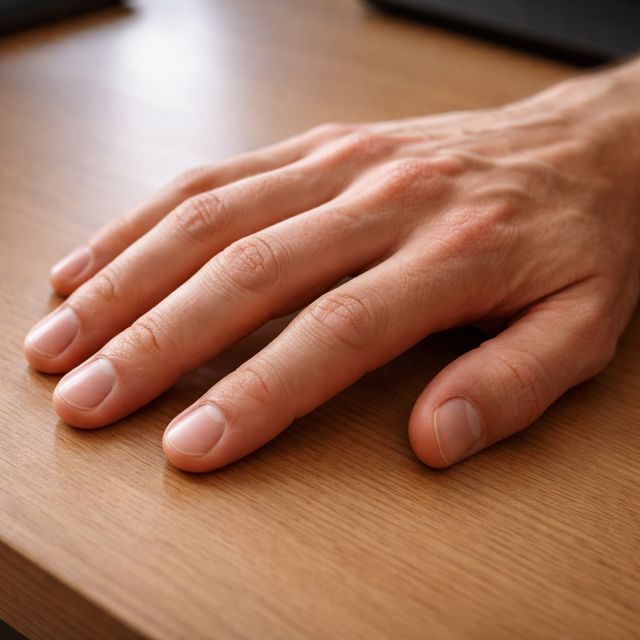
\includegraphics[width=0.102\textwidth,height=0.068\textwidth,keepaspectratio]{figures/gallery/Pair_1_commonsense.jpg} &
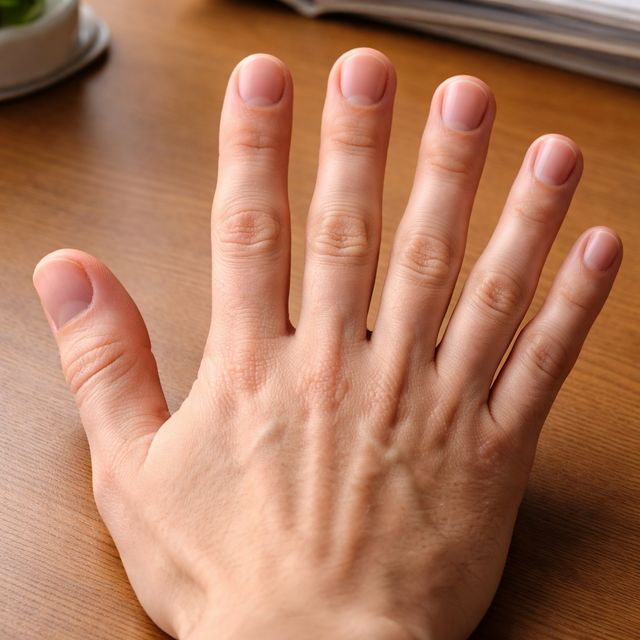
\includegraphics[width=0.102\textwidth,height=0.068\textwidth,keepaspectratio]{figures/gallery/Pair_1_counterfactual.jpg} \\
\multicolumn{2}{c}{\small Body Parts}
\end{tabular} &
\begin{tabular}{@{}cc@{}}
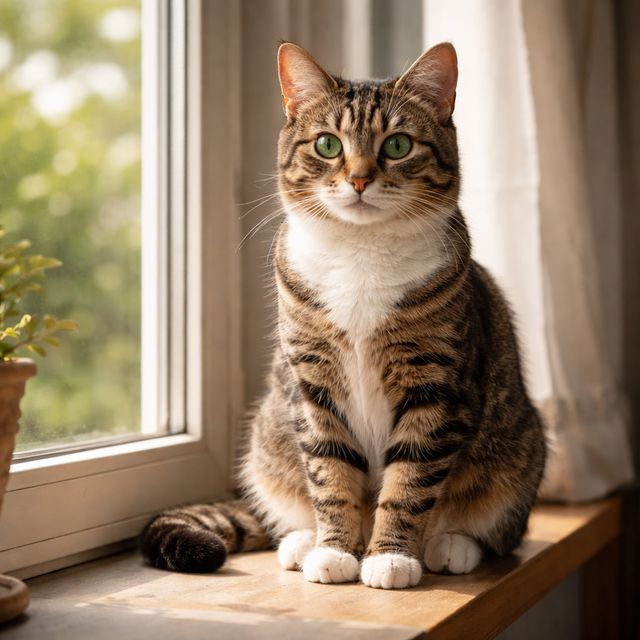
\includegraphics[width=0.102\textwidth,height=0.068\textwidth,keepaspectratio]{figures/gallery/Pair_26_commonsense.jpg} &
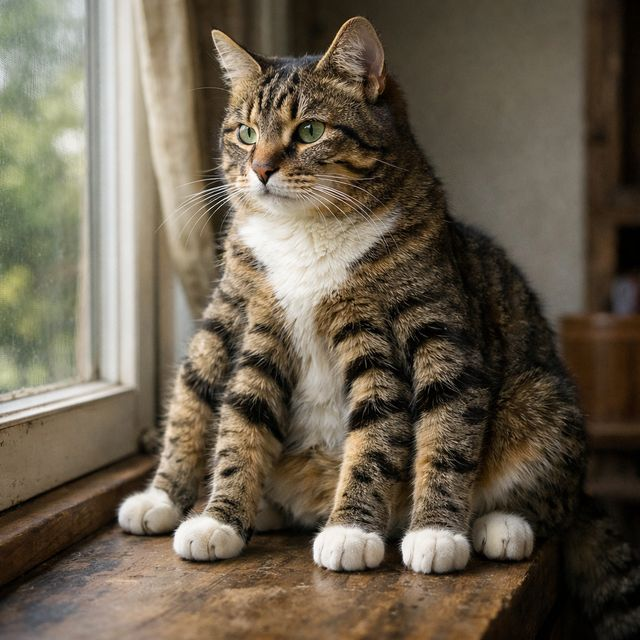
\includegraphics[width=0.102\textwidth,height=0.068\textwidth,keepaspectratio]{figures/gallery/Pair_26_counterfactual.jpg} \\
\multicolumn{2}{c}{\small Animal Parts}
\end{tabular} &
\begin{tabular}{@{}cc@{}}
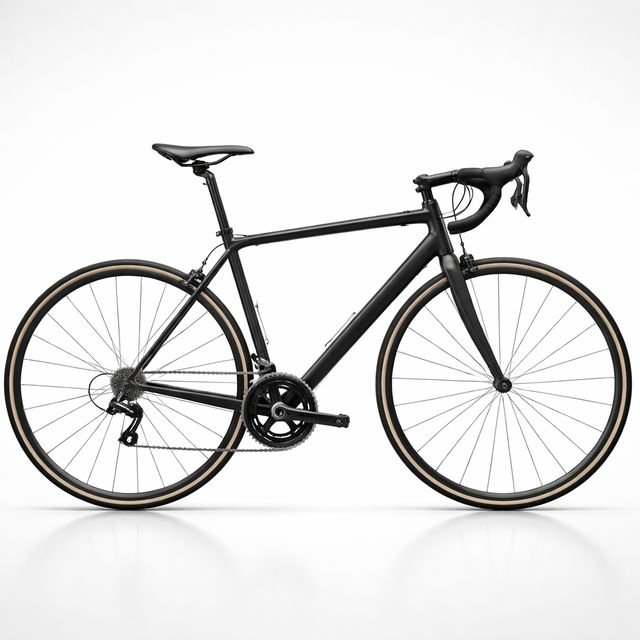
\includegraphics[width=0.102\textwidth,height=0.068\textwidth,keepaspectratio]{figures/gallery/Pair_76_commonsense.jpg} &
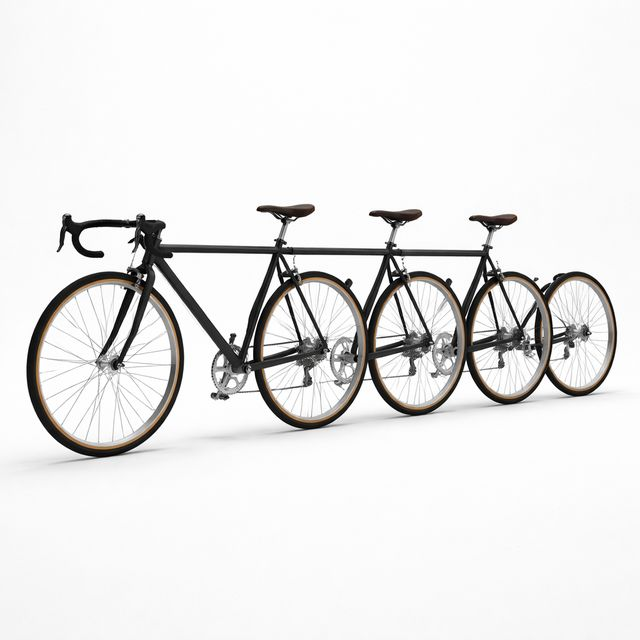
\includegraphics[width=0.102\textwidth,height=0.068\textwidth,keepaspectratio]{figures/gallery/Pair_76_counterfactual.jpg} \\
\multicolumn{2}{c}{\small Everyday Objects}
\end{tabular} &
\begin{tabular}{@{}cc@{}}

\includegraphics[width=0.102\textwidth,height=0.068\textwidth,keepaspectratio]{figures/gallery/Pair_51_commonsense.jpg} &

\includegraphics[width=0.102\textwidth,height=0.068\textwidth,keepaspectratio]{figures/gallery/Pair_51_counterfactual.jpg} \\
\multicolumn{2}{c}{\small Plant Structure}
\end{tabular}
\end{tabular}\\[3pt]
\textbf{Attribute anomalies (100 pairs)}\\
\begin{tabular}{@{}ccccc@{}}
\begin{tabular}{@{}cc@{}}
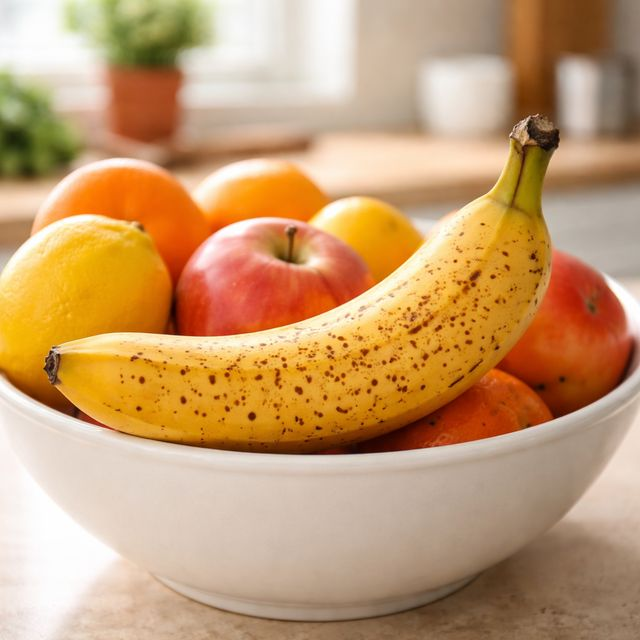
\includegraphics[width=0.081\textwidth,height=0.060\textwidth,keepaspectratio]{figures/gallery/Pair_201_commonsense.jpg} &
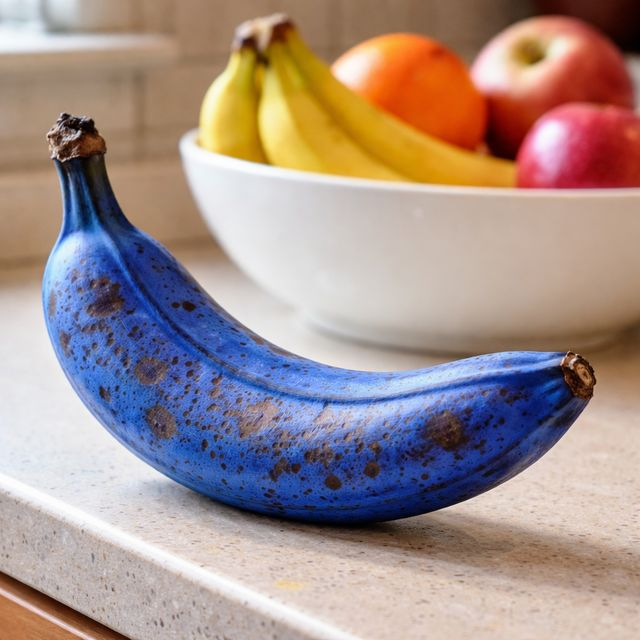
\includegraphics[width=0.081\textwidth,height=0.060\textwidth,keepaspectratio]{figures/gallery/Pair_201_counterfactual.jpg} \\
\multicolumn{2}{c}{\small Color}
\end{tabular} &
\begin{tabular}{@{}cc@{}}
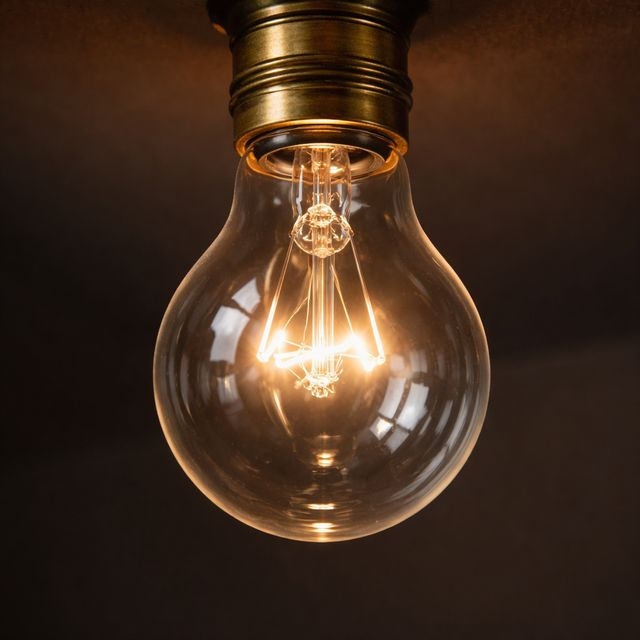
\includegraphics[width=0.081\textwidth,height=0.060\textwidth,keepaspectratio]{figures/gallery/Pair_227_commonsense.jpg} &
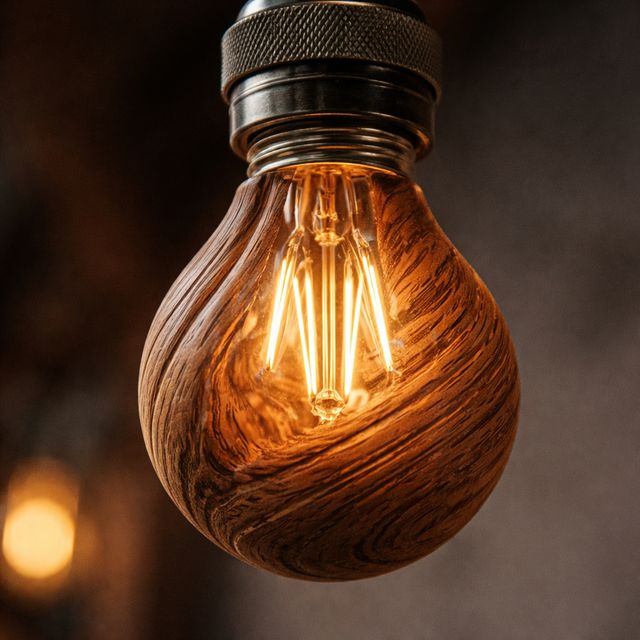
\includegraphics[width=0.081\textwidth,height=0.060\textwidth,keepaspectratio]{figures/gallery/Pair_227_counterfactual.jpg} \\
\multicolumn{2}{c}{\small Material}
\end{tabular} &
\begin{tabular}{@{}cc@{}}
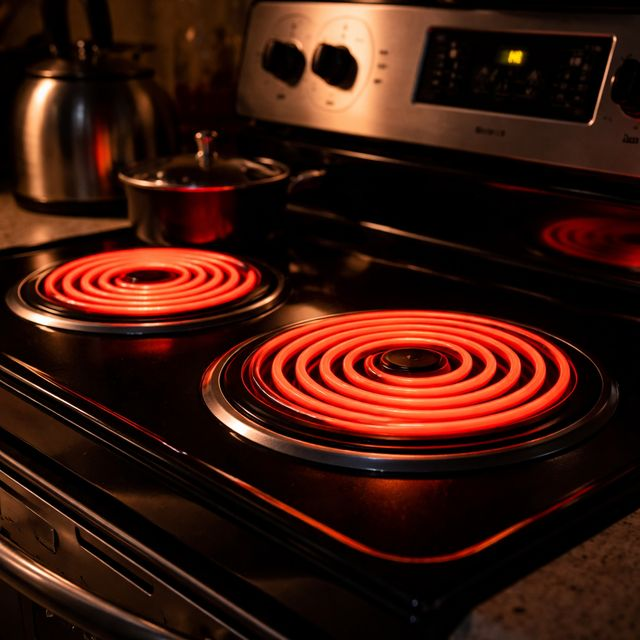
\includegraphics[width=0.081\textwidth,height=0.060\textwidth,keepaspectratio]{figures/gallery/Pair_252_commonsense.jpg} &
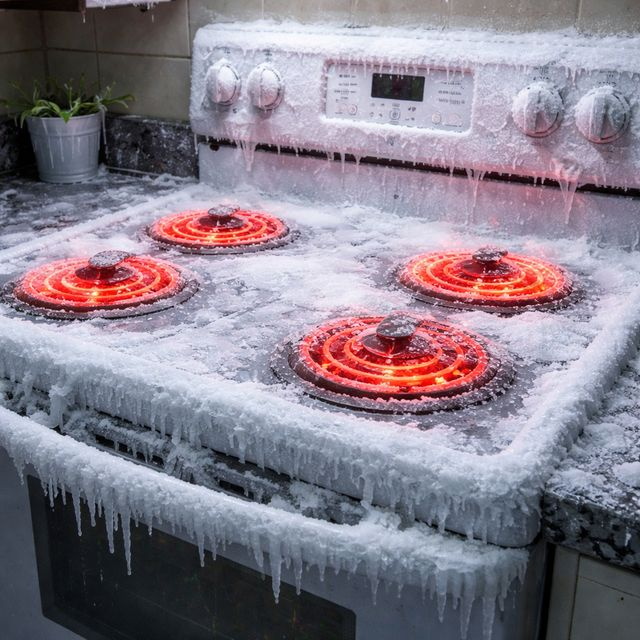
\includegraphics[width=0.081\textwidth,height=0.060\textwidth,keepaspectratio]{figures/gallery/Pair_252_counterfactual.jpg} \\
\multicolumn{2}{c}{\small Temperature}
\end{tabular} &
\begin{tabular}{@{}cc@{}}
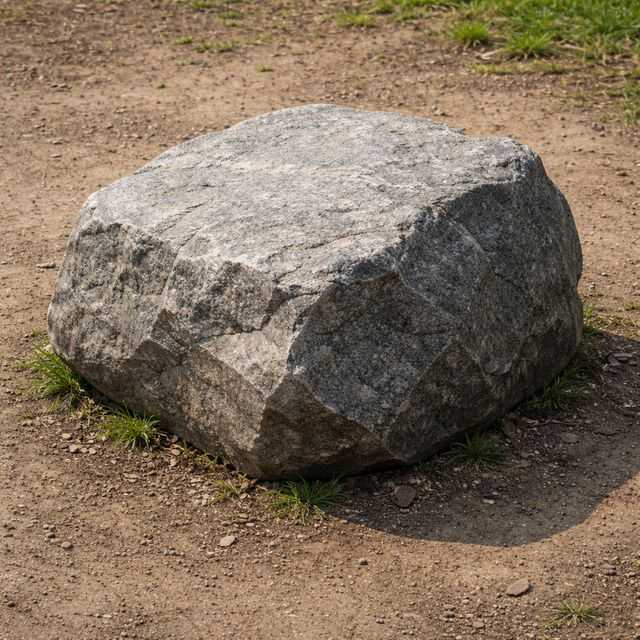
\includegraphics[width=0.081\textwidth,height=0.060\textwidth,keepaspectratio]{figures/gallery/Pair_271_commonsense.jpg} &
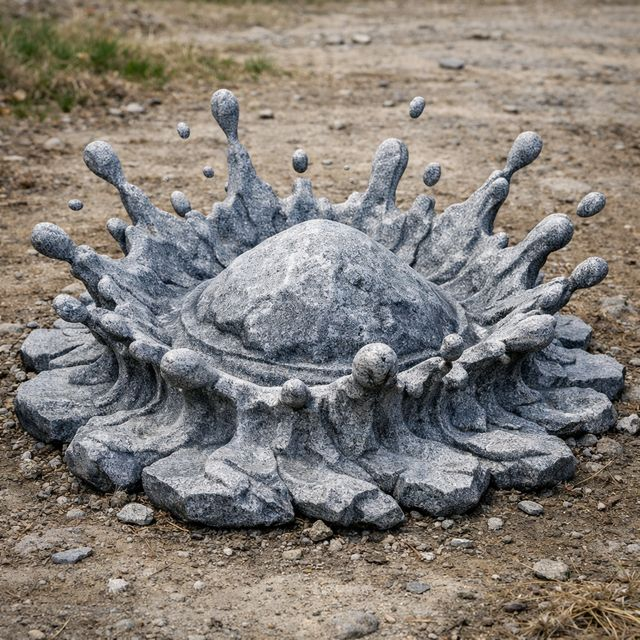
\includegraphics[width=0.081\textwidth,height=0.060\textwidth,keepaspectratio]{figures/gallery/Pair_271_counterfactual.jpg} \\
\multicolumn{2}{c}{\small Physical State}
\end{tabular} &
\begin{tabular}{@{}cc@{}}

\includegraphics[width=0.081\textwidth,height=0.060\textwidth,keepaspectratio]{figures/gallery/Pair_286_commonsense.jpg} &
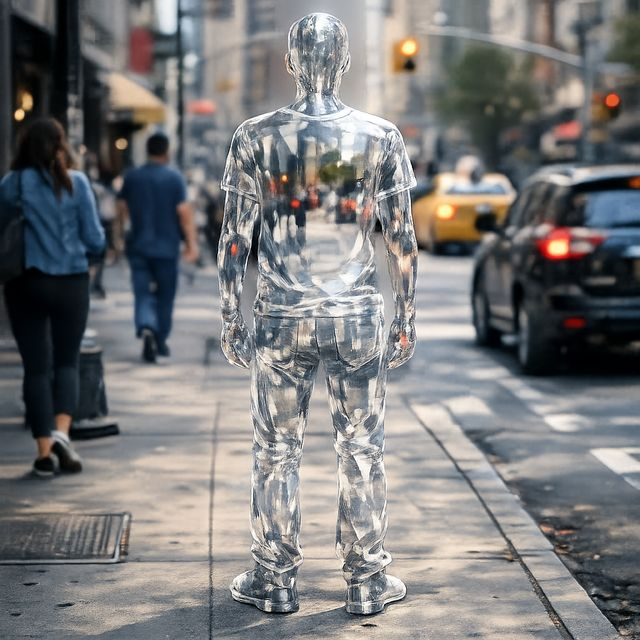
\includegraphics[width=0.081\textwidth,height=0.060\textwidth,keepaspectratio]{figures/gallery/Pair_286_counterfactual.jpg} \\
\multicolumn{2}{c}{\small Luminescence/Transparency}
\end{tabular}
\end{tabular}\\[3pt]
\textbf{Relational anomalies (100 pairs)}\\
\begin{tabular}{@{}ccccc@{}}
\begin{tabular}{@{}cc@{}}
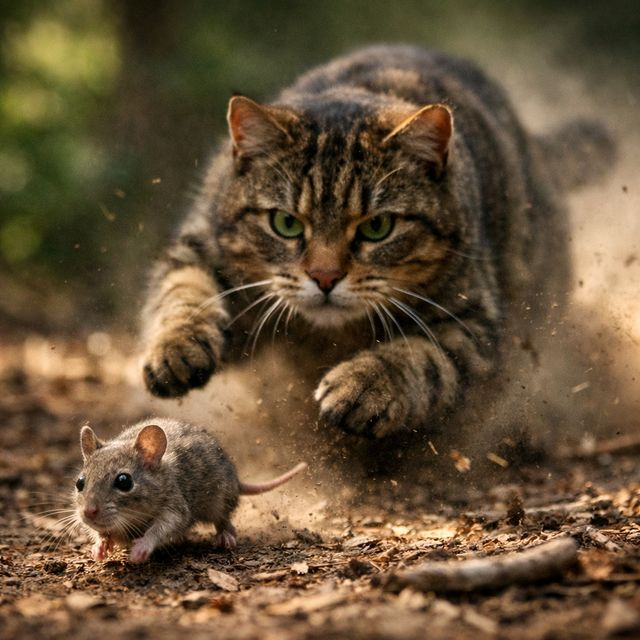
\includegraphics[width=0.081\textwidth,height=0.060\textwidth,keepaspectratio]{figures/gallery/Pair_101_commonsense.jpg} &
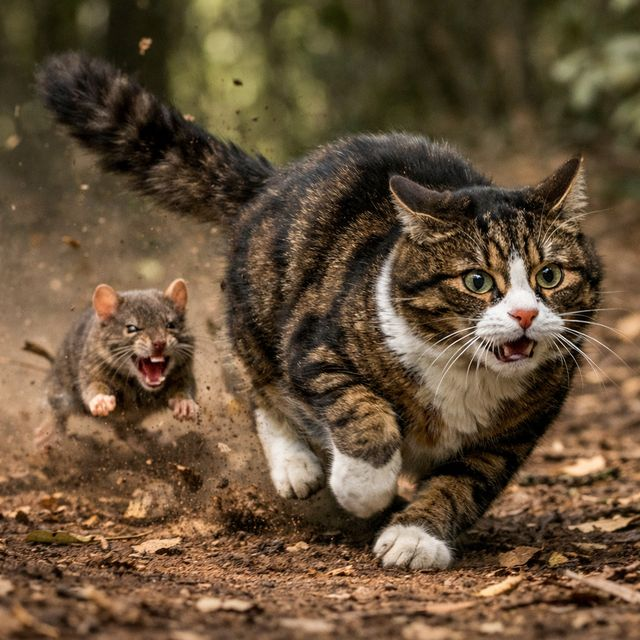
\includegraphics[width=0.081\textwidth,height=0.060\textwidth,keepaspectratio]{figures/gallery/Pair_101_counterfactual.jpg} \\
\multicolumn{2}{c}{\small Animal Behavior}
\end{tabular} &
\begin{tabular}{@{}cc@{}}

\includegraphics[width=0.081\textwidth,height=0.060\textwidth,keepaspectratio]{figures/gallery/Pair_124_commonsense.jpg} &
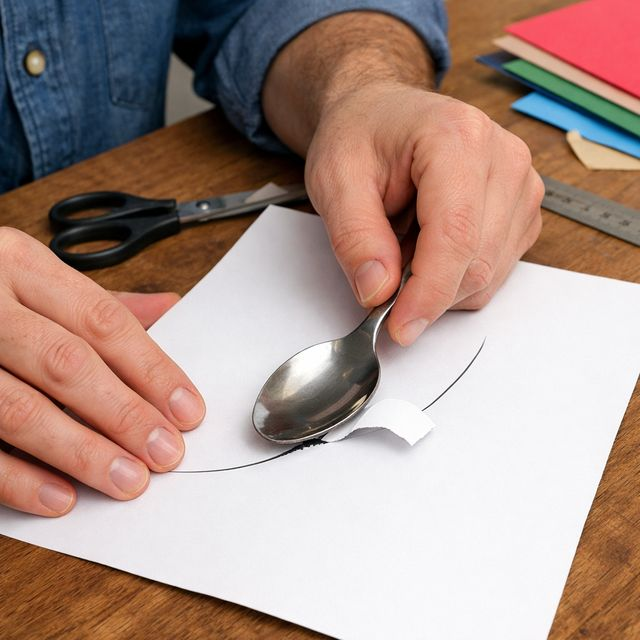
\includegraphics[width=0.081\textwidth,height=0.060\textwidth,keepaspectratio]{figures/gallery/Pair_124_counterfactual.jpg} \\
\multicolumn{2}{c}{\small Object Function}
\end{tabular} &
\begin{tabular}{@{}cc@{}}
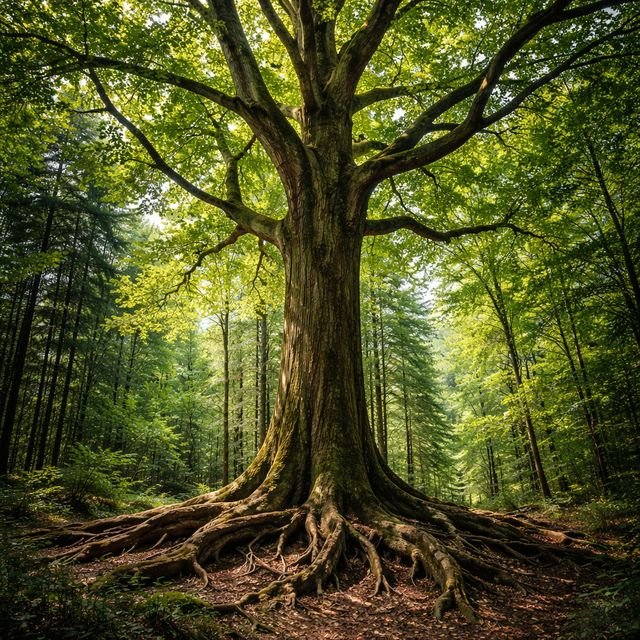
\includegraphics[width=0.081\textwidth,height=0.060\textwidth,keepaspectratio]{figures/gallery/Pair_142_commonsense.jpg} &

\includegraphics[width=0.081\textwidth,height=0.060\textwidth,keepaspectratio]{figures/gallery/Pair_142_counterfactual.jpg} \\
\multicolumn{2}{c}{\small Spatial}
\end{tabular} &
\begin{tabular}{@{}cc@{}}
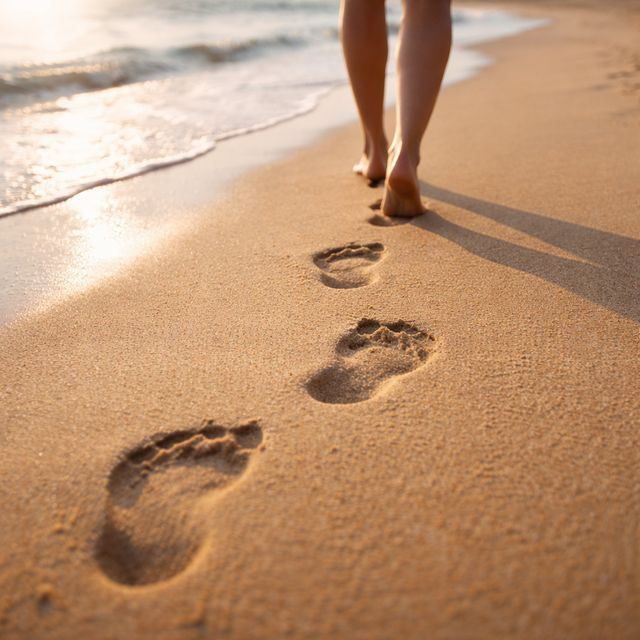
\includegraphics[width=0.081\textwidth,height=0.060\textwidth,keepaspectratio]{figures/gallery/Pair_185_commonsense.jpg} &
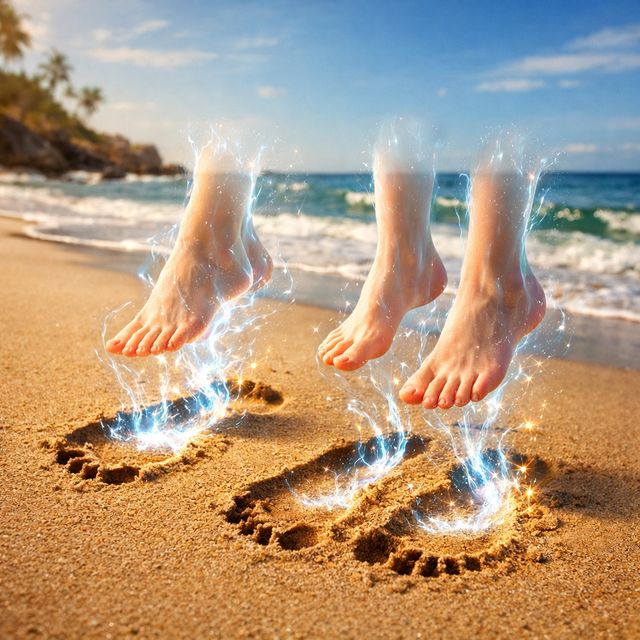
\includegraphics[width=0.081\textwidth,height=0.060\textwidth,keepaspectratio]{figures/gallery/Pair_185_counterfactual.jpg} \\
\multicolumn{2}{c}{\small Causality}
\end{tabular} &
\begin{tabular}{@{}cc@{}}
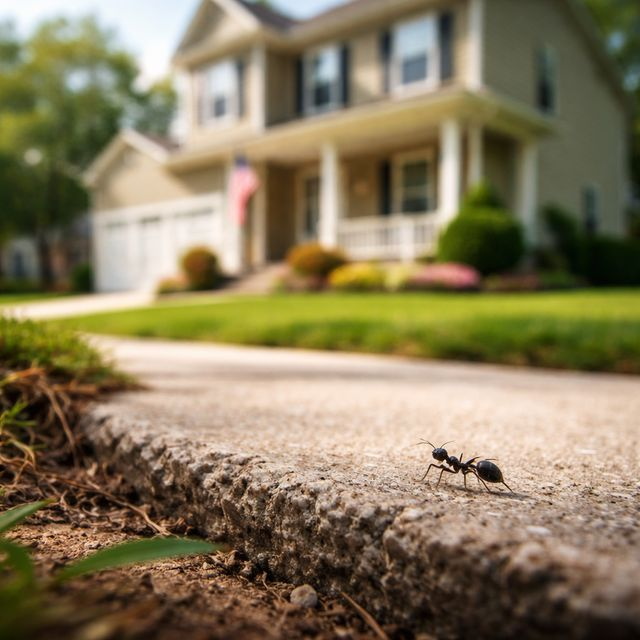
\includegraphics[width=0.081\textwidth,height=0.060\textwidth,keepaspectratio]{figures/gallery/Pair_162_commonsense.jpg} &
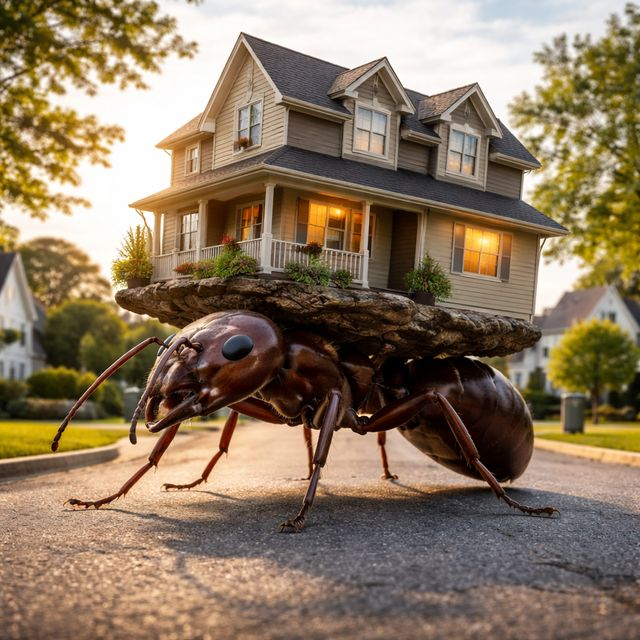
\includegraphics[width=0.081\textwidth,height=0.060\textwidth,keepaspectratio]{figures/gallery/Pair_162_counterfactual.jpg} \\
\multicolumn{2}{c}{\small Size Scale}
\end{tabular}
\end{tabular}
\caption{Representative CDH pairs from all 14 subcategories. Within every
cell, the CS control is on the left and the CF conflict is on the right. The
three families change what must be recovered from the image: cardinality,
visual attributes, or the relation between entities and events. Every test
prediction still receives only one of the two images.}
\label{fig:supp-category-gallery}
\end{figure*}

Figure~\ref{fig:supp-category-gallery} expands the benchmark view beyond a
single counting example. Counting contains four 25-pair subcategories;
attributes contain Color and Material (25 each), Temperature (20), and
Physical State and Luminescence/Transparency (15 each); relations contain five
20-pair subcategories. Pairing preserves the queried concept while reversing
whether visual evidence agrees with the ordinary-world prior, so the same
repair--retention test applies to counts, properties, interactions, causality,
scale, and spatial structure.

The primary setting is the learned route, selected under a four-point
development CS-loss budget. The CPRC+NoLan extension fills abstentions with
the released analytic proposal without overriding accepted corrections, and
CPRC-Post's posterior uncertainty check serves as a matched control; its
separately selected ten-point High-Repair setting is retained for the
attribution diagnostics.
Qwen3-VL-32B \cite{bai2025qwen3vl} and LLaVA-1.6-34B
\cite{liu2024llavabaselines} receive the complete MC, QA, stress, and transfer
matrix. Qwen3-VL-30B-A3B \cite{bai2025qwen3vl} runs an MC
replication covering signature alignment, paired repair--retention, and
leave-one-family-out transfer only.

Every row is evaluated independently. At inference, the method receives one
image, the native question, and its candidate set. The paired image and benchmark
metadata serve only to measure CF repair and CS retention. The score-geometry
features contain no task, subcategory, pair, side, or answer labels.

The QA polarity-and-template track uses native MC answer texts for 299 pairs and
the existing caption answers for the one pair with malformed MC annotations;
these construct the questions and are never side information to a method. If
$a_{\mathrm{CS}}$ and $a_{\mathrm{CF}}$ are the two mutually exclusive visual
answers, paired forms ask whether $a_{\mathrm{CS}}$ rather than
$a_{\mathrm{CF}}$ is correct and vice versa. Each image side therefore has 300
``yes'' and 300 ``no'' labels across the two forms; the 70/230 pair split is
unchanged. Four templates preserve this truth condition while varying syntax:
the original contrastive construction, \emph{instead}, a direct \emph{choice},
and explicit rejection of the second claim. CPRC is fitted only on the two
contrastive forms from 70 development pairs and applied unchanged to all four
templates on 230 unseen pairs. We report CF/CS accuracy for each form, logical
complement consistency, and joint accuracy requiring both forms to be correct.
Frozen PAI \cite{liu2024pai} and four answer-only policies (identity, always-yes, always-no, and
inversion) provide direction controls selected only on development data.

\paragraph{Single-image information boundary.}
Let $D$ denote the 70-pair development split. Every reported test prediction has
the form $f(I_i,q_i,\mathcal{Y}_i;\theta_D)$, where $\mathcal{Y}_i$ contains
only the candidates native to QA or MC. The paired image, CF/CS identity,
category, pair identifier, and test answer are outside this function. Removing
$I_i$ or deriving a degraded view from $I_i$ is a self-contrast of the same row,
not an additional visual observation. Thus pairing increases the strength of
the evaluation without making the inference problem easier.

\section{Idealized Recoverability Analysis}

Let $\mathcal{Y}$ be a finite candidate set and let centered image and prior-estimate
scores satisfy
\begin{equation}
\bar s_I(y)=v(y)+\alpha p(y)+\epsilon(y),\qquad
\bar s_P(y)=p(y).
\end{equation}
CPRC ranks $s_\lambda(y)=\bar s_I(y)-\lambda\bar s_P(y)$.
This additive form is a sufficient-condition model for understanding the
subtraction rule.

\paragraph{Proposition 1 (exact recovery).}
If $\epsilon(y)=0$ for all $y$, $\mathcal{Y}$ contains the visually correct
answer $y^*$, and $\lambda=\alpha$, then
\begin{equation}
\arg\max_y s_\lambda(y)=\arg\max_y v(y).
\end{equation}

\emph{Proof.} Substitution cancels $\alpha p(y)$ candidate by candidate, leaving
$s_\alpha(y)=v(y)$. Centering and candidate-independent constants cannot change
the ranking. \hfill(QED)

\paragraph{Proposition 2 (robust recovery interval).}
Define
\begin{align}
\Delta_v &= \min_{y\ne y^*}\bigl[v(y^*)-v(y)\bigr],\\
R_p &= \max_{y\ne y^*}|p(y^*)-p(y)|,\\
R_e &= \max_{y\ne y^*}|\epsilon(y^*)-\epsilon(y)|.
\end{align}
If $\Delta_v>R_e$, $R_p>0$, and
\begin{equation}
|\lambda-\alpha|<(\Delta_v-R_e)/R_p,
\end{equation}
then $y^*$ is the unique top candidate under CPRC.

\emph{Proof.} For every $y\ne y^*$, the corrected pairwise margin is
\begin{align}
s_\lambda(y^*)-s_\lambda(y)
&=v(y^*)-v(y)\\
&\quad +(\alpha-\lambda)[p(y^*)-p(y)]\\
&\quad +\epsilon(y^*)-\epsilon(y)\\
&\ge \Delta_v-|\lambda-\alpha|R_p-R_e>0.
\end{align}
When $R_p=0$, prior subtraction cannot alter any pairwise ranking and the
condition reduces to $\Delta_v>R_e$. \hfill(QED)

\paragraph{Corollary (when a fixed coefficient is enough).}
For sample $j$ with $R_{p,j}>0$, let
$\delta_j=(\Delta_{v,j}-R_{e,j})/R_{p,j}$ and
$A_j=(\alpha_j-\delta_j,\alpha_j+\delta_j)\cap[0,\infty)$. A single fixed
coefficient satisfies Proposition 2 for every sample exactly when
$\bigcap_j A_j$ is nonempty. If these sufficient-recovery intervals are
disjoint, no fixed coefficient can provide the same joint guarantee; a
feature-conditioned calibrator can do so when its observable contexts separate
the samples well enough to place each $\lambda_j$ inside $A_j$. This is the
formal reason to learn correction strength rather than assume that every
question absorbs the same amount of prior.

For observed scores, all inequalities
$s_\lambda(y)\ge s_\lambda(y')$ are linear in $\lambda$. Their intersection is
the exact coefficient interval over which $y$ is top-ranked. The core CPRC
proposal is defined by the fitted coefficient; the optional CPRC-Post variant
integrates posterior mass over this interval rather than treating that estimate
as certain.

\paragraph{Measured stable intervals.}
On the held-out test rows, the fitted MAP coefficient lies strictly inside its
proposal's stable interval on all 1{,}840 rows (four model--format cells),
which holds by construction and is verified numerically
(Fig.~\ref{fig:lambda-intervals}). The intervals are typically wide: median
width 1.10--1.74 across cells, with 15--51\% of rows unbounded above. The
development-selected cap respects them: $\lambda_{\max}$ does not exceed the
interval's upper end for 76.5\% (Qwen MC) to 99.6\% (LLaVA MC) of rows, and
wherever $\lambda_\theta$ touches the cap, the cap itself remains inside the
interval. Replacing $\lambda_\theta(o)$ by the dev-fitted constant $\lambda^*$
(0.80 Qwen, 0.74 LLaVA) falls outside the learned proposals' intervals on
5.9\% of Qwen and 1.1\% of LLaVA rows. The interval does not, however,
discriminate correction quality: defining the stability radius
$r=\min(\lambda-\lambda_{\mathrm{lo}},\lambda_{\mathrm{hi}}-\lambda)$, repaired
and harmed rows have nearly identical median radii (0.29 vs.\ 0.28; one-sided
Mann--Whitney $p=0.38$). Stable intervals therefore certify that overrides are
interior decisions rather than boundary instabilities, but per-row abstention
needs a signal beyond the geometry of the interval.

\begin{figure}[t]
\centering
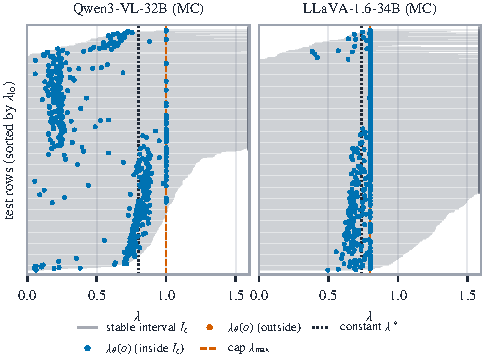
\includegraphics[width=0.9\columnwidth]{figures/lambda_stable_intervals.pdf}
\caption{\textbf{Fitted coefficients sit inside their recovery intervals.}
Each row is one unseen MC example, sorted by the interval's lower end;
segments show the proposal's stable interval (truncated at 1.6), dots the
fitted $\lambda_\theta(o)$, the dashed line the coefficient cap, and the
dotted line the dev-fitted constant $\lambda^*$.}
\label{fig:lambda-intervals}
\end{figure}

\paragraph{Proposition 3 (the repair--retention frontier).}
Suppose two samples have identical permitted inference observables
$(s_I,s_P,\phi(o))$, but the same proposed override repairs one and harms the other.
Every deterministic gate using these observables makes the same decision on
both. Repair and retention therefore form a genuine statistical frontier.
CPRC estimates that frontier from held-out calibration data and selects an
operating point through the paired CF/CS objective.

\emph{Proof.} A deterministic gate is a function of its permitted observables;
identical inputs produce the same decision, which cannot match two opposing
outcomes simultaneously. \hfill(QED)

\section{Prior-Calibrator Instantiation and Optional Bayesian Retention}

Let $K=|\mathcal Y|$, $q_I=\operatorname{softmax}(\bar s_I)$,
$q_P=\operatorname{softmax}(\bar s_P)$, and let $m_I,m_P$ be the top-two score
margins. Write $i_I,i_P,i_b$ for the image-score, prior-estimate, and native
answer indices. We express CPRC through a feature-map/calibrator interface that
can accommodate alternative implementations satisfying the single-image
boundary. The present experiments evaluate only the following low-capacity
score-only instantiation, for which $\phi$ returns
\begin{align}
u=\phi(o)=[&1,\log K/\log4,\mathsf H(q_I)/\log K,\mathsf H(q_P)/\log K,\nonumber\\
&\max q_I,\max q_P,\tanh(m_I/4),\tanh(m_P/4),\nonumber\\
&JS(q_I,q_P),\mathbf1[i_I=i_P],\nonumber\\
&\mathbf1[i_b=i_I],\mathbf1[i_b=i_P],
\tanh((m_P-m_I)/4)].
\end{align}
Here $\mathsf H$ denotes entropy and $JS$ denotes Jensen--Shannon divergence.
The coordinates are, in order: a bias term; the normalized candidate count
$\log K/\log 4$; the two views' normalized entropies; their maximum
probabilities; the tanh-compressed top-two margin of each view; the
Jensen--Shannon divergence between the views; an indicator for agreement
between the two views' winners; two indicators for agreement of the native
answer with each view's winner; and the compressed margin gap
$\tanh((m_P-m_I)/4)$. These 13 descriptors summarize candidate count, confidence, uncertainty,
image--prior disagreement, and winner consistency. They are an experimental
instantiation, not the definition of CPRC. The matched image-only control uses
the same feature interface while removing every prior-estimate-dependent coordinate.
Here
$c_\theta(u)=\min\{\operatorname{softplus}(u^\top\theta),\lambda_{\max}\}$.

For a development set $D$, CPRC uses a regularized coefficient fit with
$\theta\sim\mathcal N(0,\rho^{-1}I)$ and minimizes
\begin{equation}
\sum_{i\in D}-\log\operatorname{softmax}
  (\bar s_{I,i}-c_\theta(u_i)\bar s_{P,i})_{y_i}
  +\frac{\rho}{2}\|\theta\|_2^2.
\end{equation}
The prior precision $\rho$ is selected on the development set. The MAP point
$\hat\theta$ defines the candidate-aligned correction used by the learned MAP
route. CPRC+NoLan gives this route priority and fills its abstentions
with the released analytic proposal
$z_A=\arg\max_y\{(1+\alpha)\bar s_I(y)-\alpha\bar s_P(y)\}$ from the main
paper. The optional CPRC-Post policy adds a Laplace posterior
$N(\hat\theta,H^{-1})$, symmetrizes the Hessian
inverse, and clips covariance eigenvalues to $[10^{-8},4]$. Sixty-four-point
Gauss--Hermite quadrature integrates candidate probabilities under the induced
one-dimensional latent Gaussian. Posterior top support is computed analytically
from the intersection of all pairwise linear inequalities in $\lambda$, with
the selected cap handled as a point mass at the boundary.

For each full-matrix checkpoint, $D$ jointly contains MC and QA from the same 70
pairs: CF and CS sides contribute four rows per pair. Model selection maximizes
the mean of the two task utilities $\Delta CF+0.5\Delta CS$, requires
nonnegative development CF change in each task, and enforces the stated CS-loss
budget separately on MC and QA. The fitted coefficient is checkpoint-specific
but receives no task indicator. The sparse-MoE replication follows the same
rule on MC alone because it is an MC-only experiment.

\begin{table}[t]
\centering
\small
\setlength{\tabcolsep}{2.2pt}
\begin{tabular}{lrrrr}
\toprule
& \multicolumn{2}{c}{Primary MAP} & \multicolumn{2}{c}{High-Repair Post} \\
\cmidrule(lr){2-3}\cmidrule(lr){4-5}
Setting & Qwen & LLaVA & Qwen & LLaVA \\
\midrule
$L_2$ prior strength & 0.01 & 0.01 & 0.01 & 1.0 \\
$\lambda$ cap & 1.0 & 0.8 & 1.0 & 1.2 \\
Visual support & 0.5 & 0.5 & 0.5 & 0.5 \\
Absorption support & 0.5 & 0.5 & 0.5 & 0.5 \\
Support margin & 0.3 & 0.2 & 0.0 & 0.0 \\
Max Mahalanobis distance & $\infty$ & $\infty$ & 6.5955 & 6.3903 \\
Quadrature points & 0 & 0 & 64 & 64 \\
\bottomrule
\end{tabular}
\caption{Checkpoint-specific settings selected on development data. The
learned route uses the four-point CS budget and no posterior integration or
density cutoff; CPRC+NoLan adds the fixed analytic fallback. High-Repair
CPRC-Post uses the secondary ten-point budget.}
\end{table}

Development searches $L_2\in\{0.01,0.1,1,10\}$ and caps in
$\{0.8,1,1.2,1.5\}$ under $U_{0.5}=\Delta_{CF}+0.5\Delta_{CS}$. Visual and
absorption support use $\{0.5,0.65,0.8,0.9,0.95,1.01\}$, posterior margin uses
$\{0,0.05,0.1,0.2,0.3\}$, and Mahalanobis support uses the training 0.90/0.95/0.99
quantiles. All selected values and the fitted coefficient vector are fixed
before target evaluation. Analysis artifacts contain the fitted vectors and
covariance diagonals.

\paragraph{Inference.}
For each row, CPRC (1) records the native answer, (2) teacher-forces every native
candidate under the image and prior-estimation conditions, (3) extracts
$u=\phi(o)$ and applies the
learned prior calibrator $c_\theta(u)$, and (4) proposes the top candidate after
candidate-aligned subtraction. CPRC+NoLan retains an accepted learned
proposal and otherwise uses the released analytic proposal when it differs
from the native answer. CPRC-Post additionally integrates corrected
probabilities with 64-point Gauss--Hermite quadrature and accepts the proposal
only when its exact recoverability interval has sufficient posterior mass and
the context lies inside calibration support. Otherwise it returns the native
answer. Matched learned-route controls below isolate the residual proposal from this
optional uncertainty check.

The fixed-coefficient control replaces $\phi(o)$ by a constant, fits one
subtraction strength, and retains the same support gate. It is therefore a
strict special case of the prior calibrator. The direct-gate control instead
searches a fixed residual proposal and fits a regularized logistic acceptor to
predict whether that proposal improves the native answer from the same 13 score
features. The PAI-gate control replaces only the proposal with PAI's score rule
and uses the identical acceptor. All three controls share the joint fitting
rows, selection utility, and per-task CS constraint used by CPRC.

\subsection{The CPRC+NoLan Extension}

CPRC+NoLan evaluates NoLan's released analytic proposal
\begin{equation}
z_A=\arg\max_y\{(1+\alpha)\bar s_I(y)-\alpha\bar s_P(y)\},
\end{equation}
with $\alpha(o)$ and $\beta=0.8$ as in the main text, on every row the learned
route keeps. With $g_M$ denoting gate acceptance and $i_b$ the native answer,
the final decision is
\begin{equation}
\hat y=\begin{cases}
z_M,&g_M=1,\\
z_A,&g_M=0\ \text{and}\ z_A\ne i_b,\\
i_b,&\text{otherwise}.
\end{cases}
\end{equation}
The learned route keeps precedence wherever its gate accepts; the analytic
proposal only fills abstentions, and both proposals reuse the same image and
prior-estimation scores, so the extension adds no LVLM forward pass. A
posterior variant of the gate places a Laplace approximation
$\theta\sim\mathcal N(\hat\theta,H_\theta^{-1})$ over the calibrator parameters
and accepts a proposal only when enough posterior mass keeps it top-ranked
inside its stable interval (Gauss--Hermite quadrature, no additional LVLM
pass). The \emph{High-Repair} operating point selects the same gate family
under a relaxed ten-point development CS-loss budget and is used only for the
RQ1 attribution diagnostics.

\section{Baselines and Intervention Fidelity}

\paragraph{Conflict-specific scope and fair input.}
CHAIR measures unsupported objects in captions \cite{rohrbach2018chair}, and
POPE probes object existence \cite{li2023pope}. AMBER covers objects,
attributes, and relations \cite{wang2023amber}; MMHal-Bench evaluates free
responses \cite{sun2024mmhal}; HallusionBench combines visual illusion and
language hallucination \cite{guan2024hallusionbench}; and MME includes both
perception and cognition tasks \cite{fu2023mme}. Conflict-oriented evaluations
serve a different purpose: ROME tests reasoning beyond visual common sense
\cite{zhou2023rome}, VLind-Bench separates priors from capability
\cite{lee2025vlind}, ConflictVIS presents visual--knowledge conflicts
\cite{liu2025insight}, Visual CounterFact changes color and relative size
\cite{golovanevsky2025pixels}, and ReactBench diagnoses causal sources
\cite{zhou2026reactbench}. None uses CDH-Bench's same-concept CF/CS
repair--retention unit across counting, attributes, and relations
\cite{chen2026cdh}.

All methods executed on CDH follow the same test-input boundary. A row supplies
one image, the native question, and only those candidates naturally present in
the task. No method receives the paired control image, CF/CS identity,
subcategory or supercategory, answer, caption claim, or an MC-derived hint for
QA. Image-degraded and prior-estimation passes are transformations of the same
row, not reference observations. Hyperparameters may use the common 70-pair development
split; the 230 target pairs and leave-one-family-out target family remain
unavailable during selection.

\paragraph{Intervention coverage.}
The controlled matrix executes five intervention families: FoV-style grounding
inspired by vision--knowledge conflict analysis \cite{liu2025insight}, VCD
\cite{leng2024vcd} and MFCD \cite{liu2025mfcd} view contrast, PAI attention
guidance \cite{liu2024pai}, NoLan dynamic language-prior suppression
\cite{ren2026nolan}, and official REVIS latent steering \cite{wu2026revis}.
CausalMM \cite{zhou2025causalmm}, VLI \cite{liu2026vli}, Pixels Versus Priors
\cite{golovanevsky2025pixels}, and Arbitration Failure
\cite{nooralahzadeh2026arbitration} provide broader context on modality priors
and visual--knowledge conflict. CPRC uses the current question's
candidate-aligned textual/world-prior estimate as its subtraction direction; all
executed methods retain the same single-image test boundary.

All tunable baselines use the same 70-pair development split, utility
$U_{0.5}$, per-task four-point development CS-loss budget, and 230-pair
calibration-unseen evaluation. VCD searches
$\alpha\in\{0.5,1,1.5,2\}$, plausibility weight
$\beta\in\{0,0.1,0.3\}$, three degraded views, two gates, and margins
$\{0,0.25,0.75\}$. PAI searches guidance scale
$\gamma\in\{1.1,1.5,2\}$ at $\beta=0.1$. MFCD searches low- and high-frequency
weights in $\{0.5,1,1.5\}$, $\beta\in\{0,0.1,0.3\}$, two views per frequency
band, three gates, and the same margin set. The FoV-style grounding prompt has
no tuned parameter. NoLan keeps the release's dynamic score rule and coefficient
$\beta=0.8$, without CDH tuning. The selected Qwen settings are recorded in
\path{configs/strong_baselines_frozen_v1.json}; the complete LLaVA selections
and frozen test matrix are recorded in
\path{configs/llava_baseline_matrix_v1.json}.

The fixed FoV-style prompt asks the model to ground the decision in the single
image, silently verify the task-relevant visible property, treat ordinary
commonsense defaults as hypotheses rather than facts, and follow the image when
the two conflict. It contains no item-specific fact, answer cue, pair reference,
or benchmark-side label.

PAI, NoLan, and CPRC consume the same native image/prior-estimation candidate
likelihoods, so their score equations require no additional model forward. As an
implementation check, replaying PAI from the
shared Qwen score files exactly reproduces every setting in the dedicated Qwen
PAI sweeps. LLaVA development selects $\gamma=2.0$ for both tasks. Frozen
transfer yields +6.5/+0.9 CF/CS points on MC (18 repairs, 3 harms) and
+21.3/-4.3 on QA (51 repairs, 2 harms). This result is useful precisely because
PAI's Qwen QA change is -17.8/-0.4: a fixed prior-suppression rule can work on
one checkpoint without providing a checkpoint-stable CDH solution.

NoLan is evaluated through its released rule
$\alpha=0.8[\tanh(1/D_{\mathrm{SKL}})+1]$ and
$s=(1+\alpha)s_I-\alpha s_P$ \cite{ren2026nolan}, with symmetric KL computed on
the task-native complete-answer distribution. This is an equation-faithful
finite-answer evaluation, not an official full-vocabulary Qwen3/LLaVA-1.6 port.
For candidate ranking, division by the positive factor $1+\alpha$ makes this
exactly $s_I-\lambda_Ns_P$ with $\lambda_N=\alpha/(1+\alpha)$. Thus NoLan is a
dynamic, hand-designed member of the same prior-residual family, while CPRC
learns its coefficient from the complete score pattern and paired CF/CS rows.
On Qwen it changes MC by +10.0/-0.4 (25 CF repairs, 2 harms) and QA by
+6.5/+0.0; on LLaVA it changes MC by +7.8/+0.4 and QA by +27.0/-6.1. The result
corroborates the prior-suppression mechanism, while its checkpoint- and
format-dependent repair--retention balance motivates paired calibration and the
semantic QA stress test.
The corresponding CF repair/harm counts are 17/2, 21/3, and 64/2 for Qwen QA,
LLaVA MC, and LLaVA QA. LLaVA QA also harms 14 previously correct CS answers
without repairing any, so its released setting exceeds the four-point
development CS budget and loses 6.1 points on the unseen CS rows.

CPRC+NoLan uses that analytic rule differently: the learned route
has priority, and the analytic prediction is consulted only when the learned
route returns the native answer. This composition is fixed before test
evaluation and introduces no additional scorer call. On Qwen, it changes MC by
+9.6/-0.4 with 25 CF repairs and 3 harms, while retaining the learned route's
+22.2/-1.7 QA result exactly. On LLaVA, it changes MC by +8.3/-0.4 and QA by
+27.0/-6.1. Relative to the learned route, the fallback adds CF accuracy in
three cells and ties the fourth; it never displaces an already accepted learned
proposal. A support-gated fallback is more conservative (+8.7/+0.0 and
+22.2/-1.7 on Qwen; +7.4/-0.4 and +24.3/-5.7 on LLaVA) but filters much of the
complementary coverage, so the ungated priority composition is retained as the CPRC+NoLan
extension.

For LLaVA, the fixed FoV-style prompt changes MC by -12.6/+3.0 and QA by
-13.0/+2.2 CF/CS points. VCD selects blur with $\alpha=2.0$, $\beta=0$, and
margin 0.25 for MC, and blur-downsample with $\alpha=1.5$, $\beta=0.3$ for QA;
the frozen changes are -2.2/-2.6 and -2.2/-0.4. MFCD selects
blur-downsample/high-pass in both formats, with equal low/high weights 0.5 for
MC and 1.5 for QA. It changes MC by +2.6/-0.4 (9 repairs, 3 harms on CF) and QA
by +5.2/-0.9 (20 repairs, 8 harms on CF). The QA CF interval is
[0.009, 0.100] and its exact McNemar $p=0.0357$; the smaller MC gain is not
individually significant. Prompt inference uses the same local checkpoint
through vLLM; a nine-row overlap audit exactly matches Transformers predictions
and correctness before the full run.

Our official REVIS run imports the released PCA,
Gram--Schmidt orthogonalization, backward layer search, risk score, threshold,
and hidden-state hook \cite{wu2026revis}. Following the release, vector extraction
uses 100 records and calibration uses at most 300 records with the 85th
factual-risk percentile. The selected
Qwen and LLaVA decoder layers are 46 and 56. Main comparisons use the paper's
family coefficients, $\alpha=1.6$ for Qwen and $\alpha=1.1$ for LLaVA, with
risk scale 1.0. The repository default $\alpha=2.5$ provides an additional
sensitivity point. Our Qwen3 implementation supplies Hugging Face input formatting and
device placement while retaining the released REVIS geometry, calibration,
gate, and intervention.

\section{Additional Results}

\subsection{Which Neutral Input Best Estimates the Prior?}
\label{sec:neutral-prior-controls}

CPRC targets a textual/world-prior score, while removing the image block is
only one way to estimate it. We therefore rerun Qwen3-VL-32B with a white
image, a black image, and a pixelwise mean image built from the 140 unique
development images. The target image never enters these controls, and the
mean control uses no test image. We also test a scale-normalized coordinate
median, a fixed 0.25 shrinkage toward that median, and a candidate-wise
uncertainty-weighted version. Table~\ref{tab:neutral-prior-controls} fixes the
paper's learned-route hyperparameters and Selective Support Gate, changing
only the prior estimator.

\begin{table}[t]
\centering
\footnotesize
\setlength{\tabcolsep}{1.5pt}
{\scriptsize
\begin{tabular}{@{}lrr@{}}
\toprule
Prior estimator & MC $\Delta_{CF}/\Delta_{CS}$ & QA $\Delta_{CF}/\Delta_{CS}$ \\
\midrule
Missing image block & \textbf{+7.8/+0.4} & \textbf{+22.2/-1.7} \\
White image & +6.5/-0.9 & +15.7/-0.4 \\
Black image & +6.1/+0.0 & +14.8/+0.0 \\
Development-mean image & +3.9/+0.9 & +0.9/+0.0 \\
Scaled robust median & +6.1/-0.9 & +15.7/+0.0 \\
Core median (3 views) & +6.5/-1.3 & +16.1/-0.4 \\
Median shrinkage ($\eta=0.25$) & +7.8/+0.9 & +22.2/-2.6 \\
Uncertainty shrinkage & +7.4/+0.4 & +22.2/-2.6 \\
\bottomrule
\end{tabular}}
\caption{Neutral-input robustness on 230 unseen pairs with the published CPRC
learned route frozen. Values are accuracy changes in percentage points. Bold
marks the retained estimator.}
\label{tab:neutral-prior-controls}
\end{table}

The controls are related but not interchangeable. On unseen rows, the top
candidate agrees between the missing-image and white/black conditions on
87.4/88.0\% of examples, while white and black agree on 96.3\%. The
development-mean condition agrees with the missing-image condition on only
76.3\%, showing that average pixels are not average semantics. Most
importantly, neither robust averaging nor uncertainty-weighted shrinkage
improves CF repair under the frozen route. We therefore use missing-image
scoring for the primary method and treat disagreement among neutral controls
as an estimator-uncertainty diagnostic rather than another correction stage.

\subsection{Paired Calibration Is Part of the Intervention}

The main paper reports the MC slice of the calibration ablation.  Table
\ref{tab:paired-calibration-full} gives the complete matrix.  All three
variants use identical frozen image/prior-estimation candidate scores, the same
learned MAP coefficient family, the same $L_2$ and cap grids, and the same gate
grid.  They differ only in which development outcomes are available to the fit
and operating-point selector.  Test labels are never used for selection.

\begin{table}[t]
\centering
\small
\setlength{\tabcolsep}{2.2pt}
\begin{tabular}{lrr}
\toprule
Fit / selection & MC $\Delta$ (R/H) & QA $\Delta$ (R/H) \\
\midrule
\multicolumn{3}{l}{\itshape Qwen3-VL-32B} \\
Paired / paired & +7.83/+0.43 (21/3) & +22.17/-1.74 (53/2) \\
Paired / CF-only & +8.26/-0.87 (24/5) & +23.91/-4.35 (57/2) \\
CF-only / CF-only & +9.57/-58.70 (34/12) & +34.35/-83.04 (82/3) \\
\midrule
\multicolumn{3}{l}{\itshape LLaVA-1.6-34B} \\
Paired / paired & +6.96/-0.43 (17/1) & +23.91/-4.78 (57/2) \\
Paired / CF-only & +12.17/-1.30 (29/1) & +30.00/-9.57 (71/2) \\
CF-only / CF-only & +16.96/-38.26 (44/5) & +40.87/-79.57 (97/3) \\
\bottomrule
\end{tabular}
\caption{Paired-calibration ablation on the unseen 230-pair test set. The
paired regime requires development $\Delta CS\geq-0.04$ separately by task;
the other selectors never observe CS correctness. Each $\Delta$ entry is
$\Delta$CF/$\Delta$CS; parenthesized R/H counts CF repairs/harms.}
\label{tab:paired-calibration-full}
\end{table}

CF-only fitting turns the estimated textual prior into an almost unconditional answer
flipper.  On Qwen it harms 140 MC-CS and 202 QA-CS rows while repairing only
five and eleven; on LLaVA it harms 91 and 192 while repairing three and nine.
Paired fitting without the CS-constrained objective is much less destructive,
but still moves LLaVA from +6.96/-0.43 to +12.17/-1.30 on MC and from
+23.91/-4.78 to +30.00/-9.57 on QA.  This separates two roles of the paired
protocol: both sides shape the coefficient fit, and CS outcomes choose a
repair--retention operating point.

\subsection{Candidate Length and Score Normalization}

The teacher-forced score used throughout the paper is
\begin{equation}
s(y)=\sum_{t=1}^{|y|}\log p(y_t\mid I,q,y_{<t}),
\end{equation}
with $I$ replaced by the configured visually neutral condition for the prior
view; our default removes the image block. The scored text is the complete native
answer key (yes/no or A/B/C/D), not the option description.  Table
\ref{tab:score-normalization} audits every candidate in all 1,200 rows per
complete-evaluation checkpoint.

\begin{table}[t]
\centering
\small
\setlength{\tabcolsep}{1.7pt}
\begin{tabular}{lrrr}
\toprule
Task & Sum $\Delta$ & Mean $\Delta$ & Agreement \\
\midrule
\multicolumn{4}{l}{\itshape Qwen3-VL-32B} \\
MC & +7.83/+0.43 & +7.83/+0.43 & 100.0/100.0/100.0 \\
QA & +22.17/-1.74 & +22.17/-1.74 & 100.0/100.0/100.0 \\
\midrule
\multicolumn{4}{l}{\itshape LLaVA-1.6-34B} \\
MC & +6.96/-0.43 & +4.35/+0.87 & 100.0/96.1/97.4 \\
QA & +23.91/-4.78 & +23.04/-4.78 & 100.0/99.1/100.0 \\
\bottomrule
\end{tabular}
\caption{Sum-vs-mean candidate-score audit. Fixed agreement is prediction
agreement over 9,600 row/coefficient comparisons per model. Selected agreement
compares independently refitted learned routes on test CF/CS rows. Each
$\Delta$ is $\Delta$CF/$\Delta$CS; agreement entries give fixed/selected-CF/
selected-CS percentages.}
\label{tab:score-normalization}
\end{table}

No row contains candidates of unequal token length, image/prior-estimation token counts
always match, and stored sums equal token count times stored means.  Therefore
length cannot favor one candidate within a row.  Mean normalization can change
which LLaVA gate is selected because it rescales score geometry across rows,
but both independently selected policies retain positive MC and QA CF gains.
The residual direction itself is invariant: sum and mean predictions agree on
every fixed-$\lambda$ comparison.

\subsection{Third-Model Core MC Replication}

Qwen3-VL-30B-A3B is evaluated in BF16 with the official
\texttt{Qwen3VLMoeForConditionalGeneration} class. The core replication covers
native-error alignment, MC repair--retention, and leave-one-family-out transfer
under the same 70/230 split and four-point development budget as the learned
route.
This replication evaluates the learned route only.

\begin{table}[t]
\centering
\small
\setlength{\tabcolsep}{4.5pt}
\begin{tabular}{lrrrr}
\toprule
Evaluation & $N$ & $\Delta$CF & $\Delta$CS & CF R/H \\
\midrule
All unseen MC pairs & 230 & +9.57 & -4.35 & 24/2 \\
Attribute held out & 75 & +9.33 & -5.33 & 7/0 \\
Counting held out & 80 & +8.75 & -2.50 & 7/0 \\
Relation held out & 75 & +6.67 & +1.33 & 7/2 \\
\bottomrule
\end{tabular}
\caption{Sparse-MoE third-model replication. Each held-out fold fits only on
the other two semantic families and tests the named family. Values are points.}
\label{tab:third-model}
\end{table}

The native model makes 84 MC CF errors; 68 (80.95\%) equal its prior-estimate
top candidate, and that candidate equals the paired CS answer in 76 errors
(90.48\%).  Overall CF repair is exact-paired significant
($p=1.05\times10^{-5}$); its raw CS decrease has $p=0.0309$ but does not survive
Holm correction over the ten primary and diagnostic model/task/side endpoints.
All three unseen families retain positive CF change, extending the signature
and correction to a sparse-MoE decoder while making its larger ordinary-side
cost explicit.

\subsection{Gate, Operating-Point, and Calibration Sensitivity}

\begin{figure*}[t]
\centering
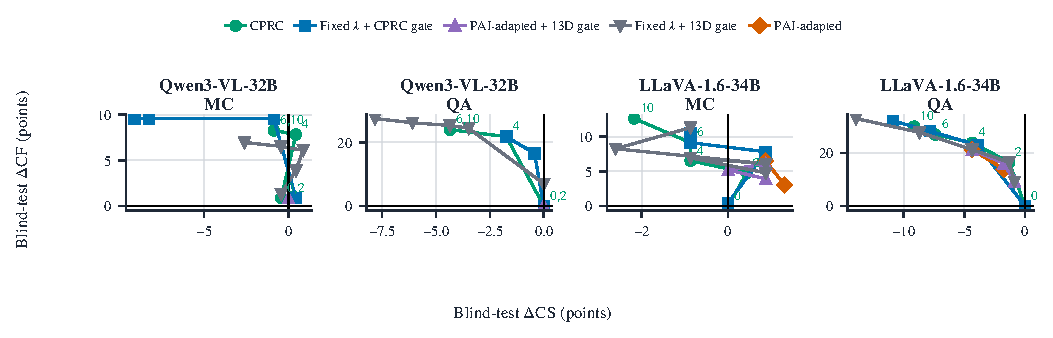
\includegraphics[width=\textwidth]{figures/gate_pareto.pdf}
\caption{Blind-test CF/CS changes after independent development selection at
CS-loss budgets of 0, 2, 4, 6, and 10 points. Learned-route annotations show the budget;
identical selected policies overlap. The fixed-$\lambda$ and PAI 13D
controls learn an override gate from the same score-distribution features and
the same 70 development pairs. The complete machine-readable frontier also
contains the 20-point budget.}
\label{fig:supp-gate-pareto}
\end{figure*}

\begin{table}[t]
\centering
\small
\setlength{\tabcolsep}{4.0pt}
\begin{tabular}{lrr}
\toprule
Method & MC & QA \\
\midrule
\multicolumn{3}{l}{\itshape Qwen3-VL-32B} \\
CPRC-Post & +7.8/+0.4 & +21.7/-1.7 \\
Learned route & +7.8/+0.4 & +22.2/-1.7 \\
\textbf{CPRC+NoLan} & \textbf{+9.6/-0.4} & \textbf{+22.2/-1.7} \\
Fixed coefficient & +9.6/-0.9 & +16.5/-0.4 \\
Direct override gate & +6.1/+0.9 & +25.2/-4.3 \\
PAI + override gate & +0.9/+0.0 & +0.0/+0.0 \\
\midrule
\multicolumn{3}{l}{\itshape LLaVA-1.6-34B} \\
CPRC-Post & +6.5/-0.9 & +23.9/-4.3 \\
Learned route & +7.0/-0.4 & +23.9/-4.8 \\
\textbf{CPRC+NoLan} & \textbf{+8.3/-0.4} & \textbf{+27.0/-6.1} \\
Fixed coefficient & +7.8/+0.9 & +23.0/-3.9 \\
Direct override gate & +6.1/+0.9 & +21.3/-4.3 \\
PAI + override gate & +6.1/+0.9 & +21.3/-4.3 \\
\bottomrule
\end{tabular}
\caption{Matched comparison at the four-point development CS-loss budget.
Each cell is $\Delta$CF/$\Delta$CS. PAI receives the same extracted score
features and logistic acceptor as the direct-gate control.}
\label{tab:matched-gate-four}
\end{table}

\begin{table}[t]
\centering
\small
\setlength{\tabcolsep}{2.1pt}
\begin{tabular}{lrrrr}
\toprule
Calibration setting & CPRC-Post & Learned route & Fixed & Direct gate \\
\midrule
\multicolumn{5}{l}{\itshape Qwen3-VL-32B} \\
Semantic holdout & 12.83 & 11.52 & 9.89 & \textbf{14.89} \\
14 pairs & 11.52 & 10.72 & 9.41 & \textbf{11.83} \\
\midrule
\multicolumn{5}{l}{\itshape LLaVA-1.6-34B} \\
Semantic holdout & 15.33 & \textbf{15.43} & 14.35 & 12.72 \\
14 pairs & 11.78 & \textbf{13.91} & 10.70 & 11.54 \\
\bottomrule
\end{tabular}
\caption{Matched utility under development shift, averaged across MC and QA as
$100(\Delta CF+0.5\Delta CS)$. Semantic holdout leaves the target
supercategory out; the 14-pair setting averages five stratified draws.}
\label{tab:matched-shift}
\end{table}

\begin{table}[t]
\centering
\small
\setlength{\tabcolsep}{3.0pt}
\begin{tabular}{lrr}
\toprule
Gate variant & MC & QA \\
\midrule
\multicolumn{3}{l}{\itshape Qwen3-VL-32B} \\
Full & +8.3/-0.9 & +23.9/-4.3 \\
No density check & +8.3/-0.9 & +23.9/-4.3 \\
No posterior check & +8.3/-0.9 & +23.9/-4.3 \\
No conflict check & +9.6/-2.6 & +22.6/-4.8 \\
Conflict only & +8.3/-0.9 & +23.9/-4.3 \\
Proposal only & +9.6/-2.6 & +22.6/-4.8 \\
Visual branch only & +0.9/-0.4 & +0.0/+0.0 \\
Prior branch only & +7.4/-0.4 & +23.9/-4.3 \\
\midrule
\multicolumn{3}{l}{\itshape LLaVA-1.6-34B} \\
Full & +12.6/-2.2 & +30.0/-9.1 \\
No density check & +12.6/-1.7 & +30.0/-9.6 \\
No posterior check & +13.0/-1.7 & +30.0/-10.0 \\
No conflict check & +11.7/-2.2 & +30.0/-9.1 \\
Conflict only & +13.0/-1.3 & +30.0/-10.4 \\
Proposal only & +12.2/-1.3 & +30.0/-10.4 \\
Visual branch only & +0.4/+0.0 & +0.0/+0.0 \\
Prior branch only & +12.2/-2.2 & +30.0/-9.1 \\
\bottomrule
\end{tabular}
\caption{Gate deletions at the frozen 10-point operating point. Each cell is
$\Delta$CF/$\Delta$CS. Branch-only rows isolate visual conflict from prior
absorption.}
\label{tab:gate-deletions}
\end{table}

Table~\ref{tab:matched-gate-four} shows that the prior-residual proposal, not
Bayesian machinery by itself, supplies most of the in-distribution gain.
The learned route closely tracks CPRC-Post, while a constant coefficient
with the same gate trades QA repair for MC repair. A separately trained 13D
override gate can buy still more Qwen QA repair, but uses the full four-point CS
budget. The complete curves reveal the complementary High-Repair boundary: at
LLaVA's ten-point setting that direct gate reaches +33.0/-13.9 QA, compared with
+30.0/-9.1 for CPRC.

Table~\ref{tab:matched-shift} makes that conclusion sharper. CPRC-Post wins over
the learned route on both Qwen shifts, but not over the direct gate; the learned route wins on
both LLaVA shifts. No uncertainty treatment is uniformly best. What survives
all four settings is the candidate-aligned residual proposal, while posterior
support changes where a checkpoint sits on the repair--retention frontier.

The selected MAP coefficient is not merely a renamed constant. On unseen Qwen
rows, its interquartile range is 0.236--0.827 for MC and 0.395--1.000 for QA;
the corresponding LLaVA ranges are 0.713--0.800 and 0.550--0.735. The LLaVA MC
distribution reaches its 0.8 cap on 62.6\% of rows, explaining why a fixed
coefficient is unusually competitive in that cell, whereas only 8.9\% of Qwen
MC rows reach their cap. Across the two semantic-holdout and two 14-pair
settings in Table~\ref{tab:matched-shift}, the stronger of the learned route and
CPRC-Post exceeds the fixed control by 1.08--3.21 utility points. Adaptivity is
therefore most visible under heterogeneous or shifted score geometry.

The deletion audit separates proposal quality from risk control. At Qwen's
selected point, density and posterior thresholds are inactive, while removing
the conflict condition spends 1.7 additional MC CS points without improving QA.
For LLaVA, dropping posterior support recovers 0.4 additional MC CF points but
increases QA CS loss from 9.1 to 10.0. More importantly, a family searched
without posterior support has no feasible LLaVA policy under the four-point
development budget. Conversely, the learned route nearly matches CPRC-Post on this
in-distribution split. We therefore interpret posterior support as
a selective risk control whose value grows under tighter or less stable
conditions. The branch audit shows that
most repairs arise in the hard prior-absorption regime where image and prior-estimate
scores initially share the native winner; direct visual conflict supplies a
smaller complementary route.

\begin{table}[t]
\centering
\small
\setlength{\tabcolsep}{1.2pt}
\begin{tabular}{lrrrr}
\toprule
Pairs & MC $\Delta$CF & MC $\Delta$CS & QA $\Delta$CF & QA $\Delta$CS \\
\midrule
\multicolumn{5}{l}{\itshape Qwen3-VL-32B} \\
14 & $+5.7\pm2.5$ & $-1.1\pm2.2$ & $+22.0\pm5.1$ & $-3.5\pm2.9$ \\
28 & $+5.7\pm2.2$ & $-2.7\pm2.0$ & $+24.1\pm3.2$ & $-4.8\pm2.7$ \\
42 & $+7.8\pm1.2$ & $-1.1\pm1.6$ & $+24.4\pm1.6$ & $-4.2\pm1.6$ \\
56 & $+8.0\pm0.5$ & $-0.3\pm0.9$ & $+23.7\pm2.2$ & $-3.9\pm1.2$ \\
70 & $+8.3\pm0.0$ & $-0.9\pm0.0$ & $+23.9\pm0.0$ & $-4.3\pm0.0$ \\
\midrule
\multicolumn{5}{l}{\itshape LLaVA-1.6-34B} \\
14 & $+4.6\pm1.0$ & $-1.0\pm0.7$ & $+26.7\pm2.6$ & $-7.0\pm1.9$ \\
28 & $+10.1\pm1.8$ & $-2.4\pm1.3$ & $+29.7\pm2.1$ & $-10.5\pm2.8$ \\
42 & $+10.0\pm1.3$ & $-1.9\pm0.8$ & $+29.5\pm2.3$ & $-10.1\pm2.9$ \\
56 & $+10.4\pm1.6$ & $-1.9\pm0.7$ & $+28.3\pm2.7$ & $-8.6\pm2.7$ \\
70 & $+12.6\pm0.0$ & $-2.2\pm0.0$ & $+30.0\pm0.0$ & $-9.1\pm0.0$ \\
\bottomrule
\end{tabular}
\caption{High-Repair calibration-size sensitivity on the fixed 230-pair test
set. For each of five seeds, subsets are nested and contain one to five pairs
from every subcategory. Cells report mean $\pm$ standard deviation in points;
the 70-pair subset is identical across seeds. Every subset is selected under the
secondary ten-point development CS-loss budget.}
\label{tab:calibration-size}
\end{table}

Even one pair per subcategory produces positive mean CF change in both formats
and models. Additional calibration most clearly strengthens MC and reduces Qwen
MC variance; QA reaches a High-Repair regime early, while its CS cost remains
checkpoint-dependent. The curve therefore separates the existence of the
prior-residual signal from the amount of data needed to stabilize its gate.

\subsection{Matched Controls and the MC-Only Calibrator}

Table~\ref{tab:controls-supp} reports controls matched to CPRC's development
data and score features: a fixed coefficient, override gates without the
learned conflict conditions, PAI proposals through the same gate, and a
calibrator fitted and selected on development MC alone. The MC-only calibrator
transfers at least as well to held-out MC as the joint MC+QA fit (+9.1 and +11.3
versus +7.8 and +7.0 CF points) and never fires on QA rows, so the joint fit
buys QA coverage rather than MC accuracy.

\begin{table}[!tb]
\centering
\footnotesize
\setlength{\tabcolsep}{2pt}
{\scriptsize
\begin{tabular*}{\columnwidth}{@{\extracolsep{\fill}}lrrrr@{}}
\toprule
Control & Qwen MC & Qwen QA & LLaVA MC & LLaVA QA \\
\midrule
CPRC-Post & +7.8/+0.4 & +21.7/-1.7 & +6.5/-0.9 & +23.9/-4.3 \\
Constant $\lambda$ & +9.6/-0.9 & +16.5/-0.4 & +7.8/+0.9 & +23.0/-3.9 \\
Direct override gate & +6.1/+0.9 & +25.2/-4.3 & +6.1/+0.9 & +21.3/-4.3 \\
PAI + override gate & +0.9/+0.0 & +0.0/+0.0 & +6.1/+0.9 & +21.3/-4.3 \\
MC-only calibrator & +9.1/-0.9 & +0.0/+0.0 & +11.3/-2.6 & +0.0/+0.0 \\
\bottomrule
\end{tabular*}}
\caption{Controls matched to CPRC's development data and score features
($\Delta$CF/$\Delta$CS in accuracy points relative to native).}
\label{tab:controls-supp}
\end{table}

\subsection{Proposal-State Decomposition of CPRC+NoLan}

Table~\ref{tab:decomposition-supp} decomposes all 1{,}840 held-out test rows by
the relationship between the learned-route and NoLan proposals. The two routes
never propose different answers: the analytic proposal only fills
learned-route abstentions, contributing 16 CF repairs against 2 harms.

\begin{table}[!tb]
\centering
\small
\setlength{\tabcolsep}{3pt}
\begin{tabular*}{\columnwidth}{@{\extracolsep{\fill}}lrrr@{}}
\toprule
Proposal state & $N$ & CF R/H & CS R/H \\
\midrule
Both routes propose the same change & 153 & 111/7 & 8/17 \\
Only the learned route proposes & 45 & 37/1 & 0/6 \\
Only the analytic rule proposes & 35 & 16/2 & 2/7 \\
Routes propose different answers & 0 & -- & -- \\
Both keep the native answer & 1{,}607 & -- & -- \\
\bottomrule
\end{tabular*}
\caption{Proposal-state decomposition of CPRC+NoLan over all 1{,}840
held-out test rows (four model--format cells pooled). R/H counts repairs and
harms under the final decision. The two routes never propose different
answers, so the analytic extension only fills learned-route abstentions.}
\label{tab:decomposition-supp}
\end{table}

\subsection{Official REVIS Direction Audit}

With the paper-family coefficients, official REVIS changes Qwen by -1.3/+0.0
points on MC and -2.2/-0.4 on QA. On LLaVA it changes MC by -1.3/+0.9 and QA by
+14.8/-3.0. All 36 changed LLaVA QA-CF answers and all seven changed QA-CS
answers move from yes to no, whereas MC repairs require different option-letter
directions. The repository coefficient 2.5 appears as an additional sensitivity
analysis.

All LLaVA QA/MC decisions are determined by the first generated token; the
generation ceiling therefore leaves the reported answer and candidate scores
unchanged.

\subsection{Original Contrastive Polarity Audit}

On native QA, the CF direction strata are highly unequal. Qwen CPRC changes
the 218 no-answer examples by +26.1 points but the 12 yes-answer examples by
-16.7; LLaVA changes them by +32.6 and -16.7. On CS, the 218 yes-answer examples
change by -4.6 and -9.6 points for Qwen and LLaVA, while neither model changes
accuracy on the 12 no-answer examples. This is why aggregate native QA cannot
establish answer-direction robustness by itself.

The balanced track reverses the two candidate answers while keeping the image
and underlying visual question fixed. With the original native MC+QA
calibration, Qwen changes ordinary-first and atypical-first CF by +37.8 and
+4.3 points; their 95\% intervals are [0.317, 0.443] and [0.013, 0.078]. A
diagnostic calibration on both balanced development forms changes them by
+36.1 and +11.7, with intervals [0.300, 0.426] and [0.074, 0.165]. LLaVA's
corresponding native-fit changes are +33.0 and -1.7 ([0.270, 0.391] and
[-0.065, 0.030]); balanced-fit changes are +46.5 and -1.3 ([0.400, 0.530] and
[-0.061, 0.035]). Thus the smaller LLaVA direction is statistically unresolved,
not evidence of a bidirectional gain. Training the gate from original MC alone
selects complete abstention on both models. The answer-only development control
also selects identity over always-yes, always-no, and inversion.

\begin{table}[t]
\centering
\small
\setlength{\tabcolsep}{3.0pt}
\begin{tabular}{llrr}
\toprule
Method & Side & Complement & Joint \\
\midrule
\multicolumn{4}{l}{\itshape Qwen3-VL-32B} \\
Native-fit CPRC & CF & 0.761$\rightarrow$0.817 & 0.448$\rightarrow$0.687 \\
 & CS & 0.983$\rightarrow$0.939 & 0.974$\rightarrow$0.913 \\
Balanced-fit CPRC & CF & 0.761$\rightarrow$0.917 & 0.448$\rightarrow$0.765 \\
 & CS & 0.983$\rightarrow$0.943 & 0.974$\rightarrow$0.926 \\
Frozen PAI & CF & 0.761$\rightarrow$0.422 & 0.448$\rightarrow$0.265 \\
 & CS & 0.983$\rightarrow$0.943 & 0.974$\rightarrow$0.935 \\
\midrule
\multicolumn{4}{l}{\itshape LLaVA-1.6-34B} \\
Native-fit CPRC & CF & 0.600$\rightarrow$0.843 & 0.304$\rightarrow$0.583 \\
 & CS & 0.922$\rightarrow$0.961 & 0.917$\rightarrow$0.948 \\
Balanced-fit CPRC & CF & 0.600$\rightarrow$0.800 & 0.304$\rightarrow$0.630 \\
 & CS & 0.922$\rightarrow$0.883 & 0.917$\rightarrow$0.870 \\
Frozen PAI & CF & 0.600$\rightarrow$0.730 & 0.304$\rightarrow$0.470 \\
 & CS & 0.922$\rightarrow$0.948 & 0.917$\rightarrow$0.939 \\
\bottomrule
\end{tabular}
\caption{Logical consistency on the 230-pair polarity test, before and after
each frozen intervention. Every cell reports before$\rightarrow$after accuracy.}
\label{tab:polarity-consistency}
\end{table}

The score views reveal where the direction asymmetry enters, before any fitted
gate is applied. Table~\ref{tab:prior-direction} asks whether each view gives
opposite predictions after the two answer claims are exchanged. The native
answer is nearly complementary on CS but substantially less so on CF. More
importantly, the textual-prior estimate is complementary on only 58.3\% of Qwen pairs
and 47.4\% of LLaVA pairs on either image side.

\begin{table}[t]
\centering
\small
\begin{tabular}{llrr}
\toprule
Model & Score view & CF comp. & CS comp. \\
\midrule
Qwen & Native & 0.761 & 0.983 \\
 & Image score & 0.378 & 0.917 \\
 & Prior estimate & 0.583 & 0.583 \\
\midrule
LLaVA & Native & 0.600 & 0.922 \\
 & Image score & 0.552 & 0.891 \\
 & Prior estimate & 0.474 & 0.474 \\
\bottomrule
\end{tabular}
\caption{Complement consistency before mitigation. A score view is
complementary when exchanging the ordinary and atypical claims exchanges its
yes/no prediction for the same image.}
\label{tab:prior-direction}
\end{table}

For ordinary-first CF questions, the textual-prior estimate favors the ordinary answer
on 99.1\% of rows for both checkpoints. Once the atypical answer is placed
first, the corresponding normal-world preference appears on only 57.4\% of
Qwen rows and 46.5\% of LLaVA rows. This loss of meaning alignment explains
why balanced development data can improve Qwen's smaller direction but cannot
make LLaVA bidirectional: in over half of the latter rows, subtraction no longer
points away from the normal-world competitor.

Frozen PAI further separates a candidate-specific correction from global prior
suppression. On Qwen its CF changes reverse from -19.1 ordinary-first to +16.5
atypical-first, and CF joint accuracy falls to 0.265. On LLaVA the same control
changes the two directions by +17.4 and +2.6 and raises joint accuracy to 0.470.
Neither global guidance nor CPRC is therefore direction-stable on every
checkpoint. On the original contrastive form, CPRC passes the stronger
bidirectional criterion on Qwen and
substantially improves complementary-pair consistency on both checkpoints; the
LLaVA result localizes the remaining QA boundary rather than averaging it away.

\subsection{Frozen Transfer Across Equivalent QA Templates}

We next ask whether the original contrastive result survives changes in wording,
not merely an exchange of answer order. Each template presents the same two
mutually exclusive visual claims without naming the CF or CS side. We fit CPRC
once on both answer orders of 70 contrastive development pairs. The policy,
feature normalization, support density, uncertainty gate, and operating point are
then frozen on 230 unseen pairs from \emph{contrastive}, \emph{instead},
\emph{choice}, and \emph{reject-second}; the last three templates are absent from
development. PAI uses one coefficient fixed on the same development split. No
test label or template-specific threshold enters either intervention.

\begin{table}[t]
\centering
\small
\setlength{\tabcolsep}{1.5pt}
\begin{tabular}{lrrrr}
\toprule
Template & Prior (\%) & CPRC O/A & PAI O/A & CF joint \\
\midrule
\multicolumn{5}{l}{\itshape Qwen3-VL-32B} \\
Contrastive & 58.3 & +36.1/+11.7 & -19.1/+16.5 & 44.8$\rightarrow$76.5 \\
Instead & 46.5 & +17.0/+10.0 & -18.7/+19.1 & 45.7$\rightarrow$63.0 \\
Choice & 52.6 & +3.0/+10.9 & -11.3/+22.2 & 54.3$\rightarrow$63.0 \\
Reject-second & 24.3 & +47.0/+1.7 & -27.8/+22.6 & 30.4$\rightarrow$65.2 \\
\midrule
\multicolumn{5}{l}{\itshape LLaVA-1.6-34B} \\
Contrastive & 47.4 & +46.5/-1.3 & +17.4/+2.6 & 30.4$\rightarrow$63.0 \\
Instead & 14.3 & +57.0/-11.3 & +18.3/-2.6 & 28.3$\rightarrow$59.1 \\
Choice & 5.7 & +21.3/-13.9 & +12.2/-10.4 & 44.3$\rightarrow$45.7 \\
Reject-second & 0.0 & +82.2/-43.0 & +29.1/-23.9 & 0.9$\rightarrow$49.1 \\
\bottomrule
\end{tabular}
\caption{Frozen transfer across semantically equivalent QA templates. Prior
complementarity is the percentage of pairs on which the prior-estimate prediction
exchanges with the claims; O/A are ordinary-/atypical-first $\Delta$CF.}
\label{tab:template-transfer}
\end{table}

Qwen improves CF in all eight template directions, while its eight CS changes
remain between -3.9 and +3.9 points. Six CF changes remain significant after
Holm adjustment over all 32 model-by-template-by-order-by-side endpoints. The
unresolved ordinary-first \emph{choice} direction is
+3.0 points ($p=0.092$, 95\% interval [0.000, 0.061]); the atypical-first
\emph{reject-second} direction is +1.7 ($p=0.557$, interval
[-0.026, 0.061]). Development selection chooses identity over always-yes,
always-no, and inversion, so the result is not reproduced by a direction-only
answer rule. Frozen PAI instead loses CF on every ordinary-first Qwen template
while gaining in every atypical-first form.

LLaVA exposes a different failure. Its prior-estimate complementarity falls from
47.4\% on the fitted wording to 14.3\%, 5.7\%, and 0.0\% on the three unseen
forms. CPRC's ordinary-first gains then coexist with atypical-first losses, and
PAI develops the same directional split. On \emph{reject-second}, CPRC changes
CF by +82.2/-43.0 and CS by -33.9/+67.8 points in O/A order. The common failure
across a candidate-specific residual and global attention guidance localizes the
problem upstream: the prior-estimation observation follows syntax without exchanging its
semantic preference. Complete repair/harm counts, paired intervals, and per-side
accuracies are retained in the released analysis artifact.

\subsection{Sample-Level Meaning-Alignment Analysis}

Template-level complementarity can hide whether the same samples carry a
usable prior direction. We partition each unseen pair before looking at model
correctness. A pair is \emph{meaning-aligned} exactly when the prior-estimate top
answer is yes for the ordinary-first question and no for the atypical-first
question. This definition uses only text-conditioned prior estimates; no
image, side label, or answer correctness enters the partition. Table
\ref{tab:semantic-conditioning-full} pools the two answer orders within each
partition, while the main paper reports them separately.

\begin{table}[t]
\centering
\small
\setlength{\tabcolsep}{1.2pt}
\begin{tabular}{lrrrrr}
\toprule
Group & $N$ & $\Delta$CF & 95\% CI & $\Delta$CS & CF;CS R/H \\
\midrule
\multicolumn{6}{l}{\itshape Qwen3-VL-32B: Contrastive} \\
Aligned & 132 & +34.47 & [28.03,41.29] & -3.79 & 91/0;0/10 \\
Other & 98 & +9.69 & [5.61,14.29] & -1.53 & 22/3;0/3 \\
\multicolumn{6}{l}{\itshape Qwen3-VL-32B: Instead} \\
Aligned & 106 & +23.58 & [17.45,30.19] & -0.47 & 50/0;0/1 \\
Other & 124 & +4.84 & [2.42,7.66] & +0.00 & 12/0;0/0 \\
\multicolumn{6}{l}{\itshape Qwen3-VL-32B: Choice} \\
Aligned & 113 & +15.49 & [11.06,20.35] & +0.00 & 35/0;0/0 \\
Other & 117 & -1.28 & [-3.42,0.43] & +0.85 & 1/4;2/0 \\
\multicolumn{6}{l}{\itshape Qwen3-VL-32B: Reject-second} \\
Aligned & 56 & +41.07 & [32.14,50.89] & -0.89 & 46/0;0/1 \\
Other & 174 & +18.97 & [14.94,22.99] & +0.29 & 77/11;10/9 \\
\midrule
\multicolumn{6}{l}{\itshape LLaVA-1.6-34B: Contrastive} \\
Aligned & 107 & +33.18 & [27.10,39.72] & -4.67 & 71/0;0/10 \\
Other & 123 & +13.41 & [8.13,18.70] & -1.22 & 51/18;10/13 \\
\multicolumn{6}{l}{\itshape LLaVA-1.6-34B: Instead} \\
Aligned & 33 & +34.85 & [24.24,45.45] & -1.52 & 23/0;0/1 \\
Other & 197 & +20.81 & [17.01,24.62] & -4.57 & 111/29;13/31 \\
\multicolumn{6}{l}{\itshape LLaVA-1.6-34B: Choice} \\
Aligned & 13 & +15.38 & [0.00,34.62] & -11.54 & 4/0;0/3 \\
Other & 217 & +3.00 & [-0.23,5.99] & -2.53 & 46/33;10/21 \\
\multicolumn{6}{l}{\itshape LLaVA-1.6-34B: Reject-second} \\
Aligned & 0 & -- & -- & -- & 0/0;0/0 \\
Other & 230 & +19.57 & [15.22,23.91] & +16.96 & 189/99;156/78 \\
\bottomrule
\end{tabular}
\caption{Sample-level semantic-equivariance conditioning. Changes and
pair-cluster intervals pool both answer orders. A/O denote aligned/other; C, I,
H, and R are the four templates. The final column gives CF;CS repairs/harms.}
\label{tab:semantic-conditioning-full}
\end{table}

Every nonempty aligned group improves both answer directions and has zero CF
harms. Pooled ``Other'' effects can nevertheless be positive because the
ordinary-first gain is much larger than the reverse-order loss. For example,
LLaVA reject-second pools to +19.57 even though its two directions are +82.17
and -43.04 points. Conditioning and direction must therefore be read together:
semantic alignment predicts a correction that follows both claims; its absence
permits a syntax-dominated one-sided gain.

\subsection{Frozen MC Option-Order Stress Test}

\begin{table}[t]
\centering
\small
\setlength{\tabcolsep}{2.0pt}
\begin{tabular}{lrrr}
\toprule
Option order & Native CF/CS & CPRC CF/CS & $\Delta$CF/CS \\
\midrule
\multicolumn{4}{l}{\itshape Qwen3-VL-32B} \\
Original & 0.665/0.965 & 0.748/0.957 & +0.083/-0.009 \\
Rotation 1 & 0.665/0.961 & 0.739/0.939 & +0.074/-0.022 \\
Rotation 2 & 0.678/0.961 & 0.757/0.922 & +0.078/-0.039 \\
Reversal & 0.687/0.970 & 0.739/0.939 & +0.052/-0.030 \\
\midrule
\multicolumn{4}{l}{\itshape LLaVA-1.6-34B} \\
Original & 0.565/0.917 & 0.691/0.896 & +0.126/-0.022 \\
Rotation 1 & 0.561/0.939 & 0.687/0.917 & +0.126/-0.022 \\
Rotation 2 & 0.530/0.943 & 0.670/0.891 & +0.139/-0.052 \\
Reversal & 0.539/0.922 & 0.674/0.878 & +0.135/-0.043 \\
\bottomrule
\end{tabular}
\caption{High-Repair MC results after remapping identical option texts and
semantics. Selection uses only the original development scores.}
\label{tab:mc-option-order}
\end{table}

At the CS-Safe point, Qwen's four CF changes range from +5.7 to +7.8 points
and its CS changes from +0.4 to -3.0; LLaVA ranges from +6.5 to +10.0 and
its CS changes from -0.9 to -2.6. At High-Repair, CPRC's absolute CF accuracy
spans only 1.7 Qwen
points and 2.2 LLaVA points across orders. Exact paired tests are adjusted as
one family of 16 model-by-order-by-side endpoints. Seven of eight CF gains
remain significant at 0.05; only Qwen reversal does not (Holm $p=0.136$).
Among CS endpoints, only LLaVA Rotate 2 remains significant
(Holm $p=0.0165$).

The stronger test also exposes a residual boundary. Native semantic predictions
are identical over all four orders on 86.5/95.2\% of Qwen CF/CS pairs and
85.2/91.3\% of LLaVA pairs; High-Repair CPRC obtains 78.7/90.9\% and
78.3/84.8\%. CPRC is therefore not exactly permutation invariant. Its narrow
accuracy range and consistently positive paired CF effect establish that the
gain survives letter changes, while these consistency rates quantify the
remaining score-order dependence.

\paragraph{Direction controls across benchmarks.}
Native CDH QA is paired visually but has 285/300 CF-no and CS-yes labels; our
stress track instead exchanges complementary claims in four forms and balances
both orders \cite{chen2026cdh}. POPE balances yes/no labels but has no matched
semantic opposite for each question \cite{li2023pope}. MME pairs positive and
negative questions that may express different propositions \cite{fu2023mme},
while HallusionBench evaluates question-pair and figure consistency without
exact direction balance \cite{guan2024hallusionbench}. ConflictVIS YN is all yes
in the 374 candidate-complete rows. Caption metrics in CHAIR
\cite{rohrbach2018chair} and free-response metrics in MMHal-Bench
\cite{sun2024mmhal} face a different omission--hallucination tradeoff. Thus balanced
labels alone do not test whether an intervention follows answer semantics.

\subsection{External Transfer Details}

\begin{table}[t]
\centering
\small
\setlength{\tabcolsep}{2.2pt}
\begin{tabular}{lrrrr}
\toprule
Track & Native & CPRC & $\Delta$ & R/H \\
\midrule
\multicolumn{5}{l}{\itshape Visual CounterFact: Qwen ($N=1{,}220$)} \\
Counterfactual & 0.962 & 0.993 & +0.031 & 38/0 \\
Commonsense & 0.998 & 0.995 & -0.002 & 2/5 \\
\multicolumn{5}{l}{\itshape Visual CounterFact: LLaVA ($N=1{,}220$)} \\
Counterfactual & 0.939 & 0.984 & +0.045 & 55/0 \\
Commonsense & 0.994 & 0.993 & -0.001 & 1/2 \\
\multicolumn{5}{l}{\itshape HallusionBench ($N=328$)} \\
Hard & 0.607 & 0.655 & +0.049 & 16/0 \\
Easy & 0.848 & 0.823 & -0.024 & 2/10 \\
\multicolumn{5}{l}{\itshape ConflictVIS ($N=374$)} \\
Multiple choice & 0.971 & 0.989 & +0.019 & 7/0 \\
Yes/no & 0.738 & 0.741 & +0.003 & 1/0 \\
\multicolumn{5}{l}{\itshape POPE ($N=3{,}000$ per split)} \\
Random & 0.917/0.911 & 0.917/0.911 & 0.000/0.000 & 0/0 \\
Popular & 0.898/0.892 & 0.898/0.892 & 0.000/0.000 & 0/0 \\
Adversarial & 0.881/0.877 & 0.881/0.877 & 0.000/0.000 & 0/0 \\
\bottomrule
\end{tabular}
\caption{External results with CDH calibration frozen. Visual CounterFact uses
the primary learned route; HallusionBench uses the explicitly secondary
High-Repair CPRC-Post policy. The analytic fallback in CPRC+NoLan is not
applied in this transfer table. Dataset headings give evaluation size. POPE
entries report accuracy/F1; all other entries report accuracy.}
\label{tab:supp-transfer}
\end{table}

Visual CounterFact \cite{golovanevsky2025pixels} supplies the most independent
paired transfer. We froze its official revision, all 1,220 color/size pairs,
A/B balancing, source hashes, and questions before running either checkpoint.
Original images form CS and the published counterfacts form CF; no
response-dependent filtering or target-label selection is performed. The
policy is selected only from the 70 CDH development pairs. The prior-estimate top
candidate is the ordinary attribute on 92.8\% of Qwen
and 82.1\% of LLaVA pairs. More diagnostically, 45 of Qwen's 46 native CF errors
and all 75 LLaVA errors match that prior-estimate candidate; all 121 errors choose the
ordinary attribute.

Under the primary learned route, Qwen changes CF/CS by +3.11/-0.25 points and LLaVA by
+4.51/-0.08. Qwen's CF interval is [0.022, 0.041] with 38/0 repairs/harms;
LLaVA's is [0.034, 0.057] with 55/0. Exact paired tests give
$p=7.28\!\times\!10^{-12}$ and $5.55\!\times\!10^{-17}$ on CF, while the
2/5 and 1/2 CS repair/harm counts are not significant. The Qwen effect is
+1.01/-0.81 on color and +4.54/+0.14 on size; LLaVA is +4.87/-0.41 and
+4.26/+0.14. Thus the learned correction transfers beyond counting, one
attribute, or one decoder family; secondary High-Repair variants are separated
below.

\begin{table}[t]
\centering
\small
\setlength{\tabcolsep}{2.0pt}
\begin{tabular}{llrr}
\toprule
Model & Frozen CDH-selected variant & $\Delta$CF & $\Delta$CS \\
\midrule
Qwen & Learned route (primary) & +3.11 & -0.25 \\
 & CPRC-Post (High-Repair) & +2.62 & -0.82 \\
 & Learned route (High-Repair) & +3.44 & -0.82 \\
 & Fixed $\lambda$ (High-Repair) & +2.38 & -0.25 \\
 & Direct gate (High-Repair) & +3.44 & -4.02 \\
LLaVA & Learned route (primary) & +4.51 & -0.08 \\
 & CPRC-Post (High-Repair) & +3.77 & +0.00 \\
 & Learned route (High-Repair) & +5.00 & +0.08 \\
 & Fixed $\lambda$ (High-Repair) & +3.93 & -0.16 \\
 & Direct gate (High-Repair) & +5.49 & -0.33 \\
\bottomrule
\end{tabular}
\caption{Frozen Visual CounterFact transfer in accuracy points. The primary
row uses the learned four-point route; all other rows are explicitly
secondary High-Repair controls. Every variant is selected on CDH development
only, and this table does not apply the analytic fallback.}
\label{tab:vcf-controls}
\end{table}

Table~\ref{tab:vcf-controls} separates the residual from its retention
machinery. Removing Laplace integration and the calibration-density cutoff does
not remove transfer; neither does replacing the adaptive coefficient with a
fixed one under the same interpretable gate. The candidate-aligned prior
residual is therefore the common correction axis. Posterior uncertainty and
the gate choose an operating point: the unconstrained direct gate is less safe
on Qwen, while the simpler learned route is stronger on this target.

The HallusionBench transfer \cite{guan2024hallusionbench} uses all 328 questions
that admit an exact easy/hard pair with opposite ground truth. With the same
BF16 checkpoint for baseline
scoring and mitigation, the frozen High-Repair CPRC-Post policy changes CF/CS
by +4.88/-2.44 points. Its 16 CF changes are all repairs
($p=0.000031$, 95\% interval [0.027, 0.073]); CS changes comprise two repairs
and ten harms ($p=0.0386$, interval [-0.046, -0.006]). Official REVIS at the paper's Qwen-family
$\alpha=1.6$ changes CF/CS by +0.61/-0.91 points, with intervals
[-0.012, 0.024] and [-0.027, 0.009]. Its risk gate is active on every row and
at 33.7\% of observed hidden positions. Both methods share the model-native BF16
baseline generations and image preprocessing.

POPE evaluation \cite{li2023pope} uses all 9,000 released questions, with
512-by-512 preprocessing shared by baseline generation and candidate scoring.
Baseline accuracy/F1 is 0.917/0.911 on random, 0.898/0.892 on popular, and
0.881/0.877 on adversarial. The CDH-fitted gate makes zero interventions in
every protocol, so all accuracy and F1 changes are 0.000. The result demonstrates
selective abstention on POPE's native binary protocol.

ConflictVIS evaluation \cite{liu2025insight} uses every candidate-complete
official row: 374 YN and 374 MC questions over 374 images, covering 171 action
and 203 place conflicts.
The open-ended SUBJ track is excluded before inference because the present
method requires a finite native candidate set. No ConflictVIS label is used for
fit or selection. On MC, whose answers span all four option letters, frozen
CPRC changes accuracy from 0.971 to 0.989 (+1.87 points; seven repairs, no
harms; $p=0.0156$; 95\% interval [0.005, 0.035]). PAI changes MC by only
+0.53 points. On YN, CPRC changes 0.738 to 0.741, while PAI changes 0.738 to
0.997. The latter gain is not balanced evidence: all 374 YN labels are yes and
ConflictVIS provides no matched ordinary-side retention control. We include it
to make the evaluation boundary explicit rather than folding a one-label score
into the paired CDH claim.

\subsection{Attribution and Generalization Details}

\paragraph{Candidate-scoring attribution.}
Replacing native generation by image-conditioned teacher-forced scoring alone
($\lambda=0$) changes Qwen by -0.9/-1.3 points on MC and -22.6/-0.4 on QA, and
LLaVA by -1.3/+1.7 and -3.5/+0.9. Thus the common candidate interface does not
explain CPRC's CF gain. Among native CF errors, the wrong answer equals the
prior-estimate top candidate in 70.1\%/90.4\% of Qwen MC/QA cases and
77.0\%/91.6\% of LLaVA cases.

\paragraph{Matched prior controls.}
\begin{table}[t]
\centering
\small
\setlength{\tabcolsep}{2.3pt}
\begin{tabular}{lrrrr}
\toprule
 & \multicolumn{2}{c}{MC} & \multicolumn{2}{c}{QA} \\
Qwen control & $\Delta$CF & $\Delta$CS & $\Delta$CF & $\Delta$CS \\
\midrule
$\lambda=0$ scorer & -0.9 & -1.3 & -22.6 & -0.4 \\
Image-only residual & 0.0 & 0.0 & 0.0 & 0.0 \\
Dev. mean & +0.4 & 0.0 & +20.9 & -5.7 \\
Shuffled (20) & -0.7$\pm$1.2 & -1.5$\pm$1.1 & +17.4$\pm$1.9 & -4.0$\pm$1.0 \\
Permuted (20) & -0.7$\pm$0.8 & -0.2$\pm$0.3 & 0.0$\pm$0.0 & 0.0$\pm$0.0 \\
\shortstack[l]{\textbf{CPRC-Post}\\\textbf{(High-Repair)}} &
\textbf{+8.3} & \textbf{-0.9} & \textbf{+23.9} & \textbf{-4.3} \\
\bottomrule
\end{tabular}
\caption{Candidate-level attribution on the 230-pair calibration-unseen split.
Stochastic controls report mean $\pm$ standard deviation over 20 fixed seeds;
values are accuracy points relative to native generation. Every row belongs to
the separately frozen secondary High-Repair suite; headline efficacy uses
the primary learned route.}
\label{tab:supp-attribution}
\end{table}

All Qwen controls refit the same score-feature CPRC instantiation with the identical
$L_2$, cap, gate, CS-constraint, and utility grids. The development-mean prior
replaces each row by the mean centered vector for its task and arity. The
shuffled control draws a same-task, same-arity donor only from development data;
the permuted control deranges candidate assignments within the current row.
Both use 20 seeds fixed in the robustness config. The image-only control reuses
the image score vector as the residual direction and zeroes every
prior-estimate-dependent context coordinate. CPRC-Post gives +8.26/-0.87 MC and
+23.91/-4.35 QA points. Mean prior gives +0.43/+0.00 and +20.87/-5.65;
shuffling gives $-0.65\pm1.22/-1.48\pm1.09$ and
$+17.35\pm1.89/-3.96\pm1.04$; permutation gives
$-0.67\pm0.80/-0.15\pm0.32$ and 0/0. Image-only is 0/0 in both tasks. Full
versus mean-prior MC has paired $p=0.00091$; every shuffled MC run is below full
with paired $p\leq0.00232$. Donor selection uses development data exclusively.

\paragraph{Unseen semantic families.}
For leave-one-family-out evaluation, each fold removes all development examples
from one of Counting, Attribute, or Relational Anomalies and evaluates only that
family in the held-out 230-pair split. Qwen obtains +8.7/+1.3 points on MC and
+24.8/-4.3 on QA; LLaVA obtains +8.7/-0.9 and +27.8/-6.1. All three held-out
families improve in both formats. In the finer 14-fold Qwen experiment, MC is
+7.0/-0.4 and QA +24.3/-3.9. MC improves/ties/falls in 9/3/2 subcategories;
QA improves/ties/falls in 13/1/0. No held-out group label enters the feature
vector or hyperparameter selection.

\begin{table}[t]
\centering
\small
\setlength{\tabcolsep}{1.6pt}
\begin{tabular}{lrrrr}
\toprule
Held-out family & MC $\Delta$ & MC R/H & QA $\Delta$ & QA R/H \\
\midrule
\multicolumn{5}{l}{\itshape Qwen3-VL-32B} \\
Attribute & +9.3/+0.0 & 7/0;1/1 & +10.7/-9.3 & 10/2;0/7 \\
Counting & +10.0/+0.0 & 8/0;1/1 & +33.8/-3.8 & 27/0;0/3 \\
Relation & +6.7/+4.0 & 7/2;3/0 & +29.3/+0.0 & 22/0;0/0 \\
\midrule
\multicolumn{5}{l}{\itshape LLaVA-1.6-34B} \\
Attribute & +5.3/+0.0 & 4/0;0/0 & +5.3/-1.3 & 6/2;0/1 \\
Counting & +10.0/-1.2 & 8/0;0/1 & +41.2/-5.0 & 33/0;0/4 \\
Relation & +10.7/-1.3 & 10/2;3/4 & +36.0/-12.0 & 27/0;0/9 \\
\bottomrule
\end{tabular}
\caption{Leave-one-family-out results in points. Each $\Delta$ cell is
$\Delta$CF/$\Delta$CS. Each R/H cell lists CF;CS repairs/harms.}
\label{tab:family-folds}
\end{table}

\begin{figure}[t]
\centering
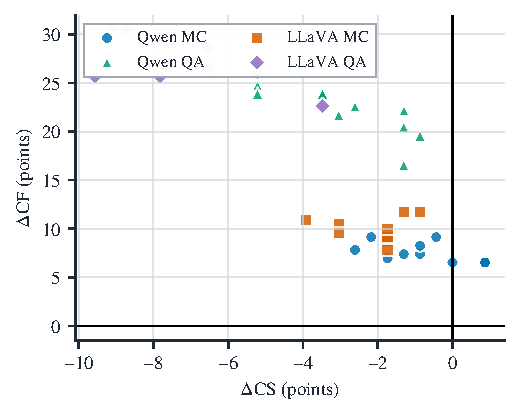
\includegraphics[width=\columnwidth]{figures/repeated_splits.pdf}
\caption{Ten metadata-stratified 70/230 splits refitted from scratch. Every
point lies above zero on the CF axis; CS variation remains visible.}
\label{fig:repeated-splits}
\end{figure}

\paragraph{Repeated stratified splits.}
We fix ten seeds before fitting. For each seed, exactly five pair IDs are
sampled from each of the 14 subcategories; both image sides and both tasks stay
in the same partition. CPRC is then refit from scratch on 70 pairs and tested
on 230. Qwen MC has $\Delta CF=+7.57\pm1.01$ and
$\Delta CS=-0.83\pm1.19$ points (ranges +6.52 to +9.13 and -2.61 to +0.87);
Qwen QA has +21.96$\pm$2.53 and -2.78$\pm$1.60 (ranges +16.52 to +24.78 and
-5.22 to -0.87). LLaVA MC has +9.96$\pm$1.27 and -2.09$\pm$0.93 (ranges +7.83
to +11.74 and -3.91 to -0.87); LLaVA QA has +27.26$\pm$2.50 and
-6.91$\pm$2.06 (ranges +22.61 to +30.43 and -9.57 to -3.48). All 40
model/task CF outcomes are positive.

\section{Statistics and Runtime}

\begin{table}[t]
\centering
\small
\setlength{\tabcolsep}{5.0pt}
\begin{tabular}{llrr}
\toprule
Model & Endpoint & Raw $p$ & Holm $p$ \\
\midrule
Qwen dense & MC CF & 0.000027 & 0.000192 \\
 & MC CS & 1.000000 & 1.000000 \\
 & QA CF & $8.55\!\times\!10^{-14}$ & $7.70\!\times\!10^{-13}$ \\
 & QA CS & 0.125000 & 0.375000 \\
LLaVA & MC CF & 0.000157 & 0.000783 \\
 & MC CS & 1.000000 & 1.000000 \\
 & QA CF & $6.00\!\times\!10^{-17}$ & $6.00\!\times\!10^{-16}$ \\
 & QA CS & 0.000122 & 0.000732 \\
Qwen sparse MoE & MC CF & 0.000010 & 0.000084 \\
 & MC CS & 0.030884 & 0.123535 \\
\bottomrule
\end{tabular}
\caption{Exact two-sided McNemar tests on the 230-pair endpoints. Dense-model
rows use CPRC+NoLan; the sparse-MoE rows use the learned route. Holm
adjustment covers the ten displayed model-by-task-by-side comparisons; QA is
diagnostic and the sparse-MoE run is MC-only.}
\label{tab:primary-holm}
\end{table}

Model generation is greedy. Each fixed configuration is evaluated once because
decoding is deterministic. We report exact repair/harm counts, exact two-sided
McNemar tests, and 10,000 pair-level bootstrap resamples with seed 20260712.
The polarity-and-template stress test uses 10,000 paired resamples with seed
20260715 and Holm adjustment over its 32 model-by-template-by-order-by-side
endpoints. Visual CounterFact uses 10,000 resamples with seed 20260715 and Holm
adjustment over its four model-by-side endpoints. Pair identity, rather than
individual image rows, is the bootstrap unit.

Experiments run on Ubuntu 22.04 with two AMD EPYC 7642 CPUs (96 physical cores),
1.0 TiB RAM, and eight 24GB RTX 3090 GPUs using driver 550.78. The software stack
uses Python 3.13.9, PyTorch 2.10.0 with CUDA 12.8, and Transformers 4.57.6. Median
serial CPRC row latency is 1.870 seconds for Qwen QA, 3.254 seconds for Qwen MC,
14.278 seconds for LLaVA QA, and 21.963 seconds for LLaVA MC. CPRC uses one
native generation and image/prior-estimation teacher-forced scoring. These conservative
timings predate shared-prefix batching; the current evaluator scores every
candidate of a view in one forward and exactly reproduces the original scores.
Posterior integration and gating add no model forwards.
The sparse-MoE core MC replication uses the batched scorer and has 1.157-second
median row latency after model loading.

\bibliography{references}

\end{document}
